%\graphicspath{{}}

\selectlanguage{french}

\begin{Article}[Titre=Minimax regret et jeu de demande 11-20,
Auteur={Gisèle Umbhauer\thanks{BETA, Université de Strasbourg. \emph{Correspondance:}
61 avenue de la Forêt Noire, 67085 Strasbourg Cedex, France. \emph{Courriel:} \href{mailto:umbhauer@unistra.fr}{umbhauer@unistra.fr}}}]

\label{UmbhauerFR}

\remerciements{Je remercie deux rapporteurs, ainsi que Jalal El Ouardighi et Bernardo Garcia-Pola pour leurs commentaires constructifs. Je remercie
également les étudiants en troisième année de licence de la Faculté des
sciences économiques et de gestion de l'Université de Strasbourg
(année universitaire 2021-2022), qui ont joué le jeu de demande 11-20.}

\begin{resume}
Le jeu de demande 11-20 d'Arad et Rubinstein stimule naturellement un
comportement conforme au raisonnement de niveau-\emph{k}. Nous montrons,
dans une version généralisée de ce jeu, que le minimax regret joue
également un rôle significatif dans le comportement induit et que la
stratégie mixte de minimax regret mime le raisonnement de
niveau-\emph{k}, dès lors que le nombre de joueurs de niveau-\emph{k}
dans une population chute avec \emph{k}. Nous montrons également qu'il
existe, pour cette famille de jeux, un lien original entre la stratégie
mixte de minimax regret et l'équilibre de Nash en stratégies mixtes, et
nous comparons les paiements obtenus avec les deux concepts.    
\end{resume}

\titrearticleENG{Minimax regret in the 11-20 money request game}

\begin{resumeENG}
Arad and Rubinstein's 11-20 money request game nicely triggers
level-\emph{k} reasoning. We show, in a general class of money-request
games, that mixed-strategy minimax regret plays a significant role too,
and that it mimics level-\emph{k} reasoning, at least if the number of
level-\emph{k} players in a population is supposed to decrease in
\emph{k}. We also show, in this class of games, an original link between
the minimax regret probability distribution and the mixed-strategy Nash
equilibrium distribution, and we compare the payoffs obtained with both
concepts.
\end{resumeENG}

\motscles{minimax regret en stratégies mixtes, raisonnement de
niveau-\emph{k}, jeu de demande 11-20, équilibre de Nash}

\keywords{mixed minimax regret, level-\emph{k} reasoning,
money-request game, Nash equilibrium}

\jelcode{C72}

\newpage

\begin{refsection}[UmbhauerFR]  

\section{INTRODUCTION}

\textcite{arad2012} ont présenté leur jeu de demande 11-20
comme le jeu qui stimule spontanément un raisonnement de
niveau-\emph{k}. Dans ce jeu à deux joueurs, chaque joueur est appelé à
demander un montant monétaire, entier naturel allant de 11 à 20. Chaque
joueur reçoit le montant qu'il demande et obtient un bonus --~montant
additionnel~-- de 20 si sa demande est juste inférieure d'une unité à la
demande de l'autre joueur.

Arad et Rubinstein ont raison, en partie du moins, d'arguer que leur jeu
(appelé <<~jeu 11-20/bonus 20~>> par la suite) est bien conçu pour étudier le
raisonnement de niveau-\emph{k}. En effet, premièrement, tout est fait
dans ce jeu pour stimuler ce type de raisonnement. Le raisonnement de
niveau-0, point d'ancrage des itérations, fait consensus~: il consiste à
jouer 20, car en jouant 20, un joueur s'assure le gain 20, qui est le
paiement maximin du jeu, ici inhabituellement élevé. Aussi un joueur qui
ne souhaite pas mener de raisonnement sophistiqué jouera sûrement 20, et
20 est donc le montant naturel pour débuter les itérations de
niveau-\emph{k}. Il s'ensuit que demander 19 est le comportement naturel
de niveau-1 (car 19 est la meilleure réponse à 20), que demander 18 est
le comportement naturel de niveau-2 (car 18 est la meilleure réponse à
19), et ainsi de suite. De plus, le conflit entre les deux acteurs est
limité, au sens où chacun obtient ce qu'il demande indépendamment du
montant demandé par l'autre; la volonté de jouer une meilleure réponse
ne devrait donc pas être entravée par des considérations sociales.
Deuxièmement, la suite des itérations de niveau-\emph{k} ne peut pas
être obtenue par d'autres types de raisonnement usuels. Il n'y a pas de
stratégie dominée dans ce jeu, aussi la dominance itérée n'a pas
d'impact; elle ne peut donc conduire au même résultat que le
raisonnement de niveau-\emph{k} (contrairement à ce qui se passe dans le
jeu de devinette -- concours de beauté -- voir \textcite{nagel1995}). Il n'y a
pas non plus d'équilibre de Nash en stratégies pures qui serait le
comportement vers lequel converge le raisonnement de niveau-\emph{k}
(contrairement au jeu de devinette). Troisièmement, le jeu est très
simple et ne demande (presque) pas de compétences cognitives pour
progresser dans la séquence des itérations. Contrairement aux jeux de
devinette, où chaque itération additionnelle nécessite le calcul d'une
nouvelle moyenne, ici chaque nouvelle itération exige uniquement de
diminuer le montant demandé de 1; la simplicité de ce calcul explique
notamment qu'une version réduite du jeu d'Arad et Rubinstein ait été
utilisée dans des expériences avec de très jeunes enfants, âgés de 5 ans
et plus (voir \textcite{fe2022}). Pour toutes ces raisons, le jeu
11-20/bonus20 semble être effectivement apte à tester le raisonnement de
niveau-\emph{k}, et plus spécifiquement la profondeur de raisonnement
des acteurs (c'est-à-dire le nombre \emph{k} d'itérations qu'ils
choisissent de mener).

Ce jeu a donné lieu à de nombreuses expériences (parmi elles \textcite{arad2012}, \textcite{lindner2013}, \textcite{goeree2018}, \textcite{li2018}, \textcite{alosferrer2021}). Certaines de ces expériences ont apporté des éclairages sur la profondeur de raisonnement et le temps de décision. Ainsi, \textcite{lindner2013} ont cherché si une contrainte temporelle pouvait
stimuler un comportement plus proche de l'équilibre de Nash\linebreak\par
\pagebreak\noindent en
stratégies mixtes et \textcite{alosferrer2021} ont étudié
le lien entre temps de décision et profondeur de raisonnement.

Toutefois le jeu d'Arad et Rubinstein a une propriété non partagée par
d'autres jeux testant le raisonnement de niveau-\emph{k}, tels les jeux
de devinette usuels. Comme cela a été observé par \textcite{li2018},
alors que les paiements des joueurs dans les jeux de devinette sont
toujours identiques (1 pour le gagnant et 0 pour les perdants), le
paiement obtenu par un joueur dans le jeu 11-20/bonus20 dépend fortement
du nombre choisi. Les gains minimaux et maximaux d'un joueur sont
croissants en fonction du montant demandé (à l'exception de 20) : un
joueur gagne au moins 19 et au plus 39 en jouant 19 alors qu'il gagne au
moins 11 et au plus 31 en choisissant 11. Ce fait peut stimuler des
traits comportementaux différents du raisonnement de niveau-\emph{k}. \textcite{li2018} ont mentionné l'aversion au risque, qui conduit
effectivement les joueurs à jouer des grands nombres plus souvent, et
\textcite{goeree2018} ont montré que la connaissance commune d'un
bruit dans le comportement mène également à jouer plus fréquemment des
grands nombres.

\enlargethispage{\baselineskip}

Dans cet article, nous arguons que le minimax regret est une autre façon
d'approcher le jeu. Le minimax regret (MR par la suite) est un concept
bien connu en théorie de la décision où il est associé à l'aversion
contre l'ambiguïté (et remonte à \textcite{savage1951} et \textcite{niehans1948}), mais il n'a été introduit que plus récemment en théorie des
jeux par \textcite{linhart1989}, \textcite{renou2010} et \textcite{halpern2012}. 
Le jeu 11-20/bonus20 comprend en effet une forte incertitude stratégique : chaque montant est rationalisable selon le concept de \textcolor{red}{Pearce [1984]} (car chaque demande \emph{x} de 11 à 19 est une meilleure réponse à la demande \(x + 1\), et 20 est la meilleure réponse à 11). D'où il est difficile d'anticiper le comportement de
l'autre joueur, et chaque décision peut générer un regret. Il découle
qu'il peut être plus raisonnable de minimiser les regrets générés plutôt
que d'essayer de répondre optimalement à une stratégie qui ne peut être
anticipée. De plus, la stratégie mixte à laquelle conduit le MR s'avère être
en accord avec la distribution de comportements générée par le
raisonnement de niveau-\emph{k}, jusqu'à une certaine profondeur de
raisonnement, si on suppose que le nombre de joueurs de niveau-\emph{k}
dans une population décroît avec \emph{k}. Ainsi le comportement issu du
raisonnement de niveau-\emph{k} peut également être obtenu en minimisant
le regret, et ce malgré que la minimisation du regret traduise une
philosophie comportementale totalement différente. \textcite{garciapola2020} a déjà observé un lien entre raisonnement de niveau-1 et MR
en stratégies pures itéré. Mais le MR en stratégies pures ne prend en
compte que les regrets maximaux, ce qui est très restrictif. Le MR en
stratégies mixtes exploite mieux tous les regrets du jeu et conduit
ainsi à un lien plus intéressant entre MR et raisonnement de
niveau-\emph{k}.

L'objectif de l'article est d'analyser ce lien ainsi que le lien entre
MR en stratégies mixtes et équilibre de Nash en stratégies mixtes, dans
une version généralisée du jeu d'Arad et Rubinstein. Nous comparons
également les gains obtenus avec le MR et l'équilibre de Nash. Enfin
nous étudions l'impact du MR dans des variantes du jeu 11-20/bonus20,
développées par \textcite{arad2012} et \textcite{goeree2018}, et nous commentons quelques traits comportementaux issus d'une expérience en classe.

En section~\ref{section:Jeu de demande exp en classe}, nous commençons par étudier brièvement comment 410~étudiants ont joué le jeu 11-20/bonus20 dans une expérience en classe menée à l'Université de Strasbourg. Cette expérience illustrera les
résultats obtenus dans les sections ultérieures. En section~\ref{section:Minimax Reg dans le jeu} nous
déterminons le comportement associé au MR en stratégies mixtes dans le
jeu 11-20/bonus20, avant d'établir ce comportement dans la version
généralisée de ce jeu. Nous montrons que la stratégie mixte qui minimise
le regret (<<~MR stratégie mixte~>> par la suite) mime une distribution
compatible avec un raisonnement de niveau-\emph{k}, quand le pourcentage
de joueurs de niveau-\emph{k} décroît avec la profondeur de
raisonnement. En section~\ref{section:Minimax Reg équilibre} nous étudions le lien original existant entre la MR stratégie mixte et l'équilibre de Nash en stratégies mixtes dans la version généralisée du jeu d'Arad et Rubinstein et nous commentons
les gains obtenus avec les deux concepts. En section~\ref{section:Commentaires sur MR} nous étudions l'impact du MR dans des variantes du jeu 11-20/bonus20. En section~\ref{section:Conclusion Umbhauer_fr} nous concluons sur des traits comportementaux observés lors de l'expérience en classe menée à Strasbourg.

\section{JEU DE DEMANDE 11-20 AVEC BONUS 20,\\ UNE EXPÉRIENCE EN CLASSE}
\label{section:Jeu de demande exp en classe}

L'expérience en classe s'est déroulée lors d'un cours de théorie des
jeux avec des étudiants en troisième année de licence de la Faculté des
sciences économiques et de gestion de l'Université de Strasbourg, durant
l'année universitaire 2021-2022. Au total 410~étudiants ont participé à
l'expérience. Les étudiants étaient homogènes en âge (entre 19 et 21~ans) et en domaine d'études (économie et gestion). Comme il est usuel
dans les expériences en classe, aucune rémunération monétaire n'a été
versée aux étudiants mais leur participation a été stimulée par une
rémunération en note de participation entrant dans la note finale à
l'examen de fin de semestre. L'expérience est un jeu joué en
\emph{one-shot}. Le jeu a été expliqué et plusieurs exemples ont été
donnés avant le début de l'expérience, pour s'assurer que les règles du
jeu soient comprises\footnote{Pour faciliter la compréhension du jeu,
  les montants étaient exprimés en euros (dans l'expérience
  d'AR [2012] les montants étaient en shekels).}. Les étudiants ont
joué le jeu avant de connaître les concepts de dominance et d'équilibre
de Nash (EN par la suite), mais ils connaissaient la notion de jeu sous
forme normale matricielle. Aussi, au moment de leur choix, ils avaient
sous leurs yeux la matrice du jeu 11-20/bonus20 (matrice~1)\footnote{Pour
  faciliter la lecture de la matrice, les gains du joueur~1 étaient
  écrits en rouge. Usuellement, dans les autres expériences portant sur
  le jeu 11-20/bonus20, les joueurs n'ont pas la matrice de paiements à
  disposition au moment du choix. Le fait de disposer de cette matrice
  peut avoir un impact sur les choix, dans la mesure où cela rend plus
  aisée la comparaison entre le gain personnel et le gain de
  l'adversaire (on reviendra sur ce fait en section~\ref{section:Conclusion Umbhauer_fr}).}.

Les étudiants devaient répondre à la question suivante :
\og{}Imaginez que vous êtes le joueur~1 et que vous êtes confronté à
un autre étudiant, le joueur~2, choisi aléatoirement dans
l'amphithéâtre. Quel montant demandez-vous~?\fg{} Ils étaient invités à
justifier leur choix par écrit.

\begin{table}[h!]
\centering
Matrice 1 : jeu 11-20/bonus20
\label{matrice1}
\resizebox{.85\linewidth}{!}{
\begin{tabular}{lc | c*{9}{c} | }
\multicolumn{12}{c}{P12} \tabularnewline % fusionner 12 cellules, centrer (c)
 & \multicolumn{1}{c}{} & 11 & 12 & 13 & 14 & 15 & 16 & 17 & 18 & 19 & \multicolumn{1}{c}{20} \tabularnewline
\cline{3-12}
& 11 & (11,11) & (31,12) & (11,13) & (11,14) & (11,15) & (11,16) &
(11,17) & (11,18) & (11,19) & (11,20) \tabularnewline
& 12 & (12,31) & (12,12) & (32,13) & (12,14) & (12,15) & (12,16) &
(12,17) & (12,18) & (12,19) & (12,20) \tabularnewline
& 13 & (13,11) & (13,32) & (13,13) & (33,14) & (13,15) & (13,16) &
(13,17) & (13,18) & (13,19) & (13,20) \tabularnewline
& 14 & (14,11) & (14,12) & (14,33) & (14,14) & (34,15) & (14,16) &
(14,17) & (14,18) & (14,19) & (14,20) \tabularnewline
Pl1 & 15 & (15,11) & (15,12) & (15,13) & (15,34) & (15,15) & (35,16) &
(15,17) & (15,18) & (15,19) & (15,20) \tabularnewline
& 16 & (16,11) & (16,12) & (16,13) & (16,14) & (16,35) & (16,16) &
(36,17) & (16,18) & (16,19) & (16,20) \tabularnewline
& 17 & (17,11) & (17,12) & (17,13) & (17,14) & (17,15) & (17,36) &
(17,17) & (37,18) & (17,19) & (17,20) \tabularnewline
& 18 & (18,11) & (18,12) & (18,13) & (18,14) & (18,15) & (18,16) &
(18,37) & (18,18) & (38,19) & (18,20) \tabularnewline
& 19 & (19,11) & (19,12) & (19,13) & (19,14) & (19,15) & (19,16) &
(19,17) & (19,38) & (19,19) & (39,20) \tabularnewline
& 20 & (20,11) & (20,12) & (20,13) & (20,14) & (20,15) & (20,16) &
(20,17) & (20,18) & (20,39) & (20,20) \tabularnewline
\cline{3-12}
\end{tabular}}
\end{table}

Les résultats de l'expérience sont donnés dans le tableau 1 et dans la
figure 1. Le tableau 1 précise également les résultats obtenus dans les
expériences d'\textcite{arad2012} (AR par la suite) et \textcite{li2018} (LR par la suite), ainsi que l'EN symétrique\footnote{Le jeu 11-20/bonus20 a d'autres EN en stratégies mixtes asymétriques, mais tous partagent la propriété que les probabilités attribuées aux montants joués décroissent avec le montant, avec une possible
  exception pour le plus bas montant joué. L'un de ces équilibres est
  tel que l'un des joueurs joue 13, 15, 17 et 19, respectivement avec
  les probabilités 8/20, 6/20, 4/20 et 2/20, alors que l'autre joueur
  joue 12, 14, 16, 18 et 20, respectivement avec les probabilités 2/20,
  7,5/20, 5,5/20, 3,5/20 et 1,5/20.} en stratégies mixtes et la MR
stratégie mixte qui sera calculée en section~\ref{section:Minimax Reg dans le jeu}.

\begin{table}[h!]
\caption{Quelques expériences du jeu 11-20/bonus20, ainsi que
  l'équilibre de Nash symétrique en stratégies mixtes et la stratégie
  mixte qui minimise le regret}\label{tabl1}
\centering
\resizebox{\linewidth}{!}{
\begin{tabular}{l    *{10}{D{6mm}}}
\toprule
Montant demandé & \centering 11 & \centering 12 & \centering 13 & \centering 14 & \centering 15 & \centering 16 & \centering 17 & \centering 18 & \centering 19 & \centering 20 \tabularnewline
\midrule
Expérience de Strasbourg (\%) & 8,3 & 0,7 & 2 & 4,4 & 4,9 & 5,9 & 14,9 &
17,5 & 28 & 13,4 \tabularnewline
Expérience AR (\%) & 4 & 0 & 3 & 6 & 1 & 6 & 32 & 30 & 12 & 6 \tabularnewline
Expérience LR (\%) & 0 & 0 & 0 & 7.3 & 1 & 4.2 & 19,8 & 37,5 & 26 &
4.2 \tabularnewline
EN symétrique (\%) & 0 & 0 & 0 & 0 & 25 & 25 & 20 & 15 & 10 & 5 \tabularnewline
MR stratégie mixte (\%) & 0 & 0 & 0 & 0 & 5 & 10 & 15 & 20 & 25 & 25 \tabularnewline
\bottomrule
\end{tabular}}
\end{table}


\begin{figure}[h]
    \centering
    \caption{Expérience en classe de l’université de Strasbourg (pourcentages) (2021/2022)}
    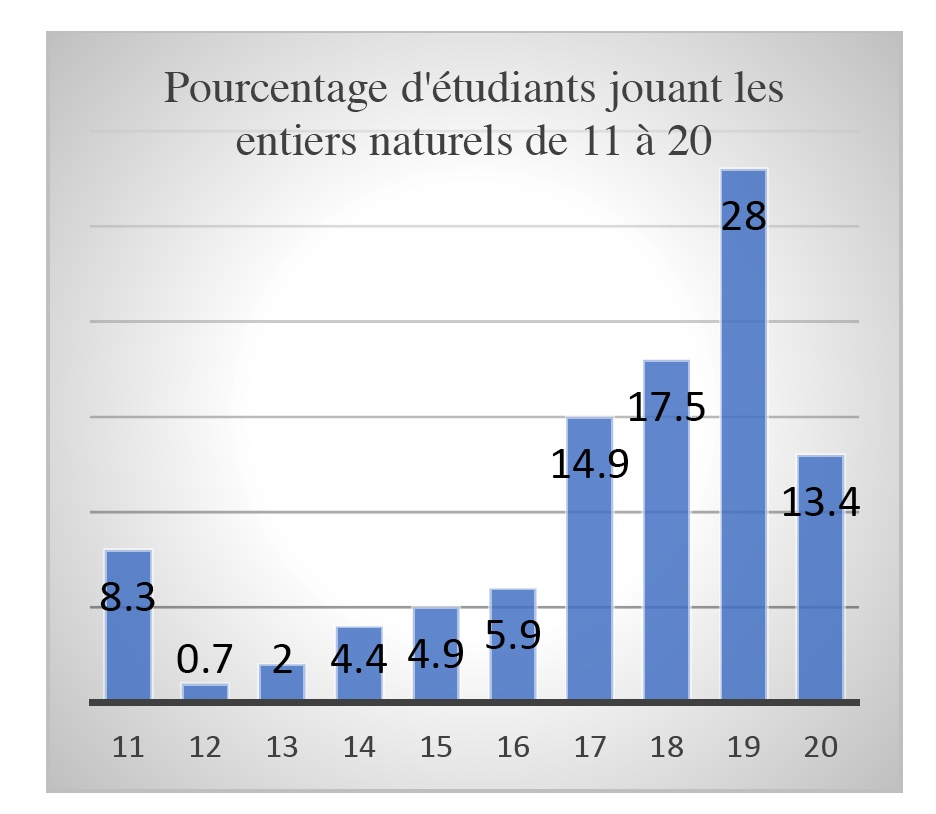
\includegraphics[height=6cm]{Articles-bons-a-composer/02_Umbhauer/02_Umbhauer_fr_Figures/02_Umbhauer_fr_figure-1.jpeg}
\end{figure}

La figure 1 est en accord avec un fait fréquemment observé dans les jeux
stimulant des raisonnements de niveau-\emph{k}, notamment les jeux de
devinette (concours de beauté), à savoir que le pourcentage de joueurs
de niveau-\emph{k} décroît avec \emph{k}, la profondeur de raisonnement
(\(k > 0\)). Ainsi 28~\% des étudiants de Strasbourg choisissent 19 (le
montant de niveau-1), 17,5~\% d'entre eux jouent 18 (raisonnement de
niveau-2), 14,9~\% d'entre eux jouent 17 (raisonnement de niveau-3) et
ainsi de suite jusqu'à 12 (voir le tableau 1). Seule l'observation que 8,3~\%
des étudiants jouent 11 n'est pas en accord avec ce fait. Cette
décroissance régulière de 19 à 12 n'est pas toujours observée dans les
autres expériences portant sur le jeu 11-20/bonus20. Ainsi 19 n'est pas
toujours le mode statistique de la distribution : c'est le cas chez \textcolor{red}{Alos-Ferrer et Buckenmaier [2018]}, mais chez AR [2012] c'est 17 et chez \textcite{lindner2013}, \textcite{goeree2018} et \textcite{li2018} c'est 18.
Plus généralement les distributions de comportements varient selon les
études\footnote{Par exemple un test du khi-deux, même restreint aux
  distributions sur les entiers de 16 à 19, montre que la distribution
  d'AR (108 joueurs) est significativement différente de celle obtenue
  dans l'expérience en classe de Strasbourg (410~joueurs) ($p<0,001$). La distribution de Strasbourg est plus proche de celle
  obtenue par \textcolor{red}{Alos-Ferrer et
  Buckenmaier [2018]} (128~joueurs), si on
  exclut les joueurs jouant 17, très peu nombreux chez Alos-Ferrer et
  Buckenmaier: les deux distributions, restreintes aux entiers 16, 18,
  19 et 20, ne sont pas significativement différentes ($p=0,14$).}
mais elles partagent toutes la propriété que les pourcentages
décroissent de 18 (ou 17 chez AR) à 14 au moins (de toute façon les
pourcentages d'acteurs demandant 11, 12, 13 sont généralement faibles).
Et toutes les distributions empiriques diffèrent profondément de l'EN
symétrique en stratégies mixtes (la valeur \emph{p} des tests du
khi-deux peut être approximée par 0).

\section{MINIMAX REGRET DANS LE JEU DE DEMANDE 11-T\\ AVEC BONUS B}
\label{section:Minimax Reg dans le jeu}

Nous abordons maintenant le MR et appliquons ce concept à une version
généralisée du jeu d'Arad et Rubinstein, le jeu 11-T/bonus\emph{B,} \emph{i.e.}
le jeu de demande 11-\emph{T} avec bonus \emph{B}, où
\(B \geq T > 11 + n\), \emph{n} étant l'entier naturel défini par :
\(n(n + 1)/2\  \leq B < (n + 1)(n + 2)/2\) (\(B = T = 20\) et \(n = 5\)
dans le jeu d'Arad et Rubinstein).

Le concept de MR est bien connu en théorie de la décision avec
incertitude et remonte à \textcite{savage1951} et \textcite{niehans1948}. Un
agent économique, lorsqu'il ne lui est pas possible d'anticiper le futur
état du monde (état de la Nature) peut opter pour une décision qui
minimise son regret, à savoir la différence entre le gain généré par sa
décision et le gain obtenu avec la meilleure décision dans l'état du
monde finalement réalisé. Le MR peut notamment partiellement expliquer
le comportement des acteurs dans le paradoxe d'\textcite{ellsberg1961}. Dans
un jeu, les joueurs ne sont pas confrontés à la Nature ou à des loteries
--~du moins pas exclusivement~-- mais à d'autres joueurs. Ils peuvent
toutefois être confrontés à une forte incertitude stratégique au sens où
il peut s'avérer difficile, pour de multiples raisons, d'anticiper
comment les autres acteurs vont jouer. Dans un tel contexte, minimiser
le regret peut s'avérer plus optimal que de jouer une meilleure réponse
à un profil de stratégies complètement inconnu.

Dans un jeu, le concept de MR en stratégies pures est défini ainsi. Soit
un jeu sous forme normale avec \emph{N} joueurs \emph{i}, des ensembles
de stratégies pures \emph{S\textsubscript{i}} et des fonctions d'utilité
\emph{u\textsubscript{i}, i} de 1 à \emph{N\textsubscript{~}}; le regret
du joueur \emph{i} lorsqu'il joue la stratégie pure\({\ \ s}_{i}\ \)et
que les autres joueurs jouent les stratégies pures
$s_{-i}$ est
\(r_{i}(s_{i},~s_{-i}) = \max_{\sigma_{i} \in S_{i}}{u_{i}\left( \sigma_{i},~s_{-i} \right) - u_{i}\left( s_{i},s_{- i} \right)}\).
Le regret maximal lié à \emph{s\textsubscript{i}} est\linebreak
\(R_{i}\left( s_{i} \right) = \max_{s_{-i} \in S_{-i}}{r_{i}(s_{i},~s_{-i})}\).
Le MR en stratégies pures du joueur \emph{i} est\linebreak
\(\min_{s_{i} \in S_{i}}{R_{i}\left( s_{i} \right)}\) (voir \textcite{linhart1989}, \textcite{renou2010} et \textcite{halpern2012}, pour plus de détails).

Ainsi le regret induit par le choix d'une stratégie, étant donné la
stratégie d'un adversaire, est la différence entre le gain obtenu avec
la meilleure réponse à la stratégie de l'adversaire et le gain réalisé
grâce à la stratégie choisie. Par exemple, dans le jeu 11-20/bonus20, si
le joueur~1 demande 14 alors que le joueur~2 demande 17, la meilleure
réponse du joueur~1 est 16 et donc son regret, $r(14, 17)$, vaut
$36-14=22$. Le regret maximal auquel conduit le montant 14, $R(14)$,
est obtenu quand le joueur~2 joue 20, auquel cas la meilleure réponse
est 19, d'où le regret maximal associé à 14 : $39-14=25$.

La matrice des regrets du joueur 1 dans le jeu 11-20/bonus20 est la
matrice 2. Le regret maximal induit par chaque montant \emph{m},
\(R(m),\ m\) de 11 à 20, y est écrit en gras.

\begin{table}[h!]
\centering
Matrice 2 : matrice des regrets du joueur 1 dans le jeu 11-20/bonus20 \par
\vspace{0.2cm}
\label{matrice2}
\resizebox{.55\linewidth}{!}{
\begin{tabular}{lc | c*{9}{c} | }
\multicolumn{12}{c}{P12} \tabularnewline
& \multicolumn{1}{l}{} & 11 & 12 & 13 & 14 & 15 & 16 & 17 & 18 & 19 & \multicolumn{1}{l}{20} \tabularnewline
\cline{3-12}
& 11 & 9 & 0 & 21 & 22 & 23 & 24 & 25 & 26 & 27 & \textbf{28} \tabularnewline
& 12 & 8 & \emph{19} & 0 & 21 & 22 & 23 & 24 & 25 & 26 & \textbf{27} \tabularnewline
& 13 & 7 & 18 & \emph{19} & 0 & 21 & 22 & 23 & 24 & 25 & \textbf{26} \tabularnewline
& 14 & 6 & 17 & 18 & \emph{19} & 0 & 21 & \emph{22} & 23 & 24 & \emph{\textbf{25}} \tabularnewline
Pl1 & 15 & 5 & 16 & 17 & 18 & 19 & 0 & 21 & 22 & 23 & \textbf{24} \tabularnewline
& 16 & 4 & 15 & 16 & 17 & 18 & \emph{19} & 0 & 21 & 22 & \textbf{23} \tabularnewline
& 17 & \ul{3} & \ul{14} & \ul{15} & \ul{16} & \ul{17} & \ul{18} &
\emph{\ul{19}} & \ul{0} & \ul{21} & \textbf{\ul{22}} \tabularnewline
& 18 & \ul{2} & \ul{13} & \ul{14} & \ul{15} & \ul{16} & \ul{17} &
\ul{18} & \emph{\ul{19}} & \ul{0} & \textbf{\ul{21}} \tabularnewline
& 19 & 1 & 12 & 13 & 14 & 15 & 16 & 17 & 18 & \emph{\textbf{19}} & 0 \tabularnewline
& 20 & 0 & 11 & 12 & 13 & 14 & 15 & 16 & 17 & 18 & \emph{\textbf{19}}
\tabularnewline
\cline{3-12}
\end{tabular}}
\end{table}

Cette matrice met en évidence les caractéristiques des regrets. Les
regrets en italique, égaux à 19, expriment que si les deux joueurs
demandent \emph{x}, alors chaque joueur regrette de ne pas avoir demandé
\(x - 1\): il aurait gagné ce faisant le montant additionnel \(B - 1\)
(\emph{B} étant le bonus égal à 20 dans le jeu d'Arad et Rubinstein).
Les regrets dans la dernière colonne sont les regrets dont souffre un
joueur lorsqu'il joue \emph{x} différent de 19 et que son adversaire
joue 20. Moins son montant demandé \emph{x} est élevé et plus ses
regrets sont grands, car il souffre à la fois de pas avoir obtenu le
bonus 20 et de la différence \(19 - x\).

La matrice est très régulière en structure. Sur une même ligne \emph{x}
(le montant demandé par le joueur 1) les regrets augmentent en fonction
du montant y demandé par l'adversaire (joueur 2) jusqu'à \(y = x\), et
croissent à nouveau de \(y = x + 2\) à \(y = 20\). Sauf pour \(x = 19,\)
le regret maximal \(R(x)\) est toujours obtenu dans la dernière colonne,
lorsque l'adversaire joue 20. Cela tient au fait que le regret dans
cette colonne, lorsqu'il n'est pas nul, vaut \(B + 19 - x,\) alors que
dans la colonne \emph{y}, pour \(11 < y < 20\), le regret ne vaut que
\(B + y - 1 - x\), nécessairement inférieur.

\textcite{garciapola2020} a observé que le MR en stratégies pures dans ce
jeu, qui vaut 19, est obtenu pour \(x = 19\) et \(x = 20\), et qu'une
application itérée du concept de MR en stratégies pures (voir \textcite{halpern2012}) conduit au choix de 19. En comparant ce résultat à ceux
induits par le raisonnement de niveau-\emph{k}, il en a conclu que, dans
ce jeu, le MR et le raisonnement de niveau-1 conduisent à demander le
même montant 19.

Nous allons plus loin dans cet article en nous tournant vers le MR en
stratégies mixtes, un concept qui prend en considération tous les
regrets de la matrice~2 (et non pas exclusivement les regrets maximaux
écrits en gras). Soient \emph{x} et \emph{y} les montants
joués respectivement par le joueur~1 et le joueur~2 (l'adversaire). Les
regrets dans chaque ligne \emph{x} croissent régulièrement en \emph{y} car ils
sont égaux à \(y - 1 + B - x\ \)(excepté pour \(y = x + 1\)). En
comparant deux lignes adjacentes \emph{x} et \(x + 1\) (par exemple les
lignes soulignées 17 et 18), on observe que les regrets du joueur~1 sont
toujours plus faibles dans la ligne \(x + 1\) que dans la ligne~\emph{x}, sauf lorsque le joueur~2 joue \(x + 1\) (dans ce cas, le
regret du joueur~1 est nul s'il joue \emph{x} et vaut 19 s'il joue
\(x + 1\)). Ce fait exprime que le joueur~1 regrette l'unité de monnaie
qu'il perd délibérément et systématiquement en jouant \emph{x} au lieu
de \(x + 1\), sauf si l'autre joueur, par chance, joue \(x + 1\). Des
observations similaires peuvent être faites en comparant deux colonnes
adjacentes, \emph{y} et \(y + 1\) (par exemple les colonnes encadrées 17
et 18). Cette fois, les regrets de la colonne \(y + 1\) excèdent
systématiquement d'une unité ceux de la colonne \emph{y}, car ils
passent de \(B + y - 1 - x\) à \(B + y - x\). Les regrets dans une même
colonne, lorsque l'adversaire joue \emph{y}, sont régulièrement
décroissants en \emph{x} (excepté en \(x = y - 1\)). Cela découle du
fait que le regret \(B + y - 1 - x\ \)peut être scindé en deux : le
regret dont souffre le joueur 1 quand il demande 20, \(y - 1 + B - 20\)
auquel s'ajoute le regret de ne pas avoir joué 20, \(20 - x\), excepté
pour \(x = y - 1\). Aussi les regrets dans la colonne \emph{y} sont
décroissants en \emph{x} car \(20 - x\) est décroissant en \emph{x}.

Ces faits conduisent intuitivement à la conjecture suivante : le concept
de regret devrait accorder une probabilité plus grande aux montants plus
élevés. Cette conjecture va s'avérer exacte.

Nous travaillons avec la notion de regret en stratégies mixtes de \textcite{renou2010}. L'idée est de construire une stratégie mixte qui
minimise le regret, noté \emph{z}, quel que soit le montant demandé par
l'adversaire. En notant \emph{p\textsubscript{t}} la probabilité du
joueur 1 de demander \emph{t}, cela revient à résoudre le programme
d'optimisation suivant~:

\newpage
%
\[
\min_{z\ p_{11}p_{12}p_{13}p_{14}p_{15}p_{16}p_{17}p_{18}p_{19}p_{20}}z
\]
s.c.
\begin{multline}
9p_{11} + 8p_{12} + 7p_{13} + 6p_{14} + 5p_{15} + 4p_{16} + 3p_{17} + 2p_{18} + 1p_{19} + 0p_{20} \leq z \\
0p_{11} + 19p_{12} + 18p_{13} + 17p_{14} + 16p_{15} + 15p_{16} + 14p_{17} + 13p_{18}
+ 12p_{19} + 11p_{20} \leq z \\
21p_{11} + 0p_{12} + 19p_{13} + 18p_{14} + 17p_{15} + 16p_{16} + 15p_{17} + 14p_{18}
+ 13p_{19} + 12p_{20} \leq z \\
22p_{11} + 21p_{12} + 0p_{13} + 19p_{14} + 18p_{15} + 17p_{16} + 16p_{17} + 15p_{18}
+ 14p_{19} + 13p_{20} \leq z \\
23p_{11} + 22p_{12} + 21p_{13} + 0p_{14} + 19p_{15} + 18p_{16} + 17p_{17} + 16p_{18}
+ 15p_{19} + 14p_{20} \leq z \\
24p_{11} + 23p_{12} + 22p_{13} + 21p_{14} + 0p_{15} + 19p_{16} + 18p_{17} + 17p_{18}
+ 16p_{19} + 15p_{20} \leq z \\ \tag{1}
25p_{11} + 24p_{12} + 23p_{13} + 22p_{14} + 21p_{15} + 0p_{16} + 19p_{17} + 18p_{18}
+ 17p_{19} + 16p_{20} \leq z \\
26p_{11} + 25p_{12} + 24p_{13} + 23p_{14} + 22p_{15} + 21p_{16} + 0p_{17} + 19p_{18}
+ 18p_{19} + 17p_{20} \leq z \\
27p_{11} + 26p_{12} + 25p_{13} + 24p_{14} + 23p_{15} + 22p_{16} + 21p_{17} + 0p_{18}
+ 19p_{19} + 18p_{20} \leq z \\
28p_{11} + 27p_{12} + 26p_{13} + 25p_{14} + 24p_{15} + 23p_{16} + 22p_{17} + 21p_{18}
+ 0p_{19} + 19p_{20} \leq z \\
p_{11} + p_{12} + p_{13} + p_{14} + p_{15} + p_{16}{+ p}_{17} + p_{18} + p_{19} + p_{20} = 1 \\
0 \leq p_{t}\enskip \text{de 11 à 20.}
\end{multline}

La résolution de ce programme conduit aux probabilités \(p_{i} = 0\), \emph{i}
de 11 à 14, $p_{15} = \frac{1}{20}, p_{16} = \frac{2}{20}, p_{17} = \frac{3}{20}, p_{18} = \frac{4}{20}, p_{19} = \frac{5}{20}, p_{20} = \frac{5}{20}$.
Le MR vaut $z=315/20=15,75$. La distribution des probabilités est
donnée en figure~2 et dans le tableau 1. En comparant les figures~1 et
2, on constate que le comportement des étudiants de l'expérience en
classe de Strasbourg est assez proche de la MR distribution, si on
exclut les fréquences avec lesquelles les étudiants jouent les montants
20 et 11, qui sont respectivement très inférieur et très supérieur à
5/20 et 0. Cela est confirmé par un test du khi-deux : si on se
restreint aux montants de 15 à 19, la distribution expérimentale n'est
pas significativement différente de la distribution obtenue avec 410
joueurs jouant la MR stratégie mixte ($p = 0,25$). Par opposition, il
est immédiat que la distribution expérimentale est significativement
différente de la distribution de l'EN symétrique donnée en figure 3 et
dans le tableau~1 (la valeur \emph{p} peut être approximée par 0, même
si on se concentre sur un nombre limité de montants).

Le résultat obtenu dans le jeu d'Arad et Rubinstein se généralise aux
jeux de demande 11-\emph{T}/bonus\emph{B}, où \(B \geq T > 11 + n\),
\emph{n} étant l'entier naturel défini par
\(n(n + 1)/2\  \leq B < (n + 1)(n + 2)/2\).

\newpage

\begin{figure}[h]
    \centering
    \caption{Stratégie mixte qui minimise le regret}
    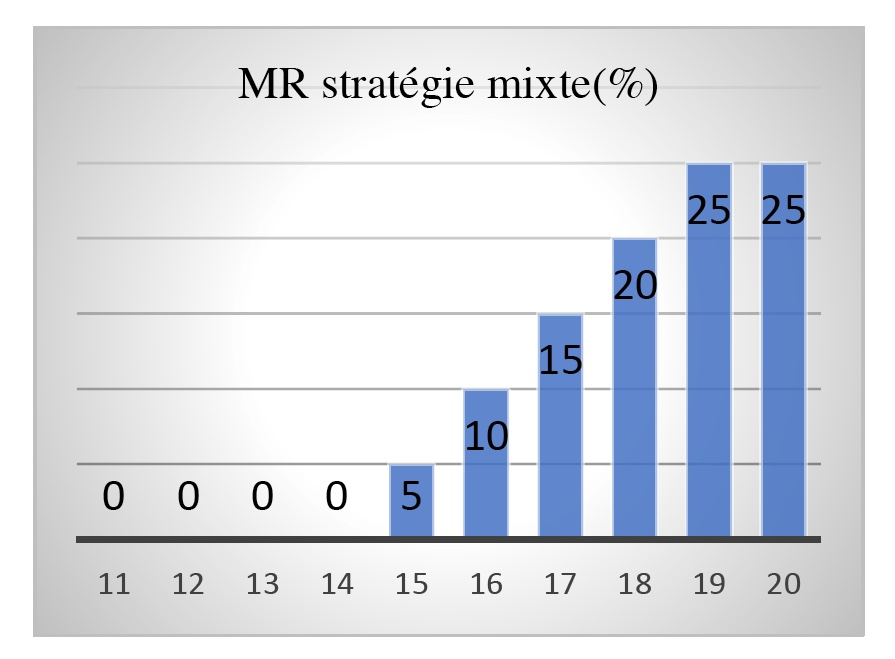
\includegraphics[height=5cm]{Articles-bons-a-composer/02_Umbhauer/02_Umbhauer_fr_Figures/02_Umbhauer_fr_figure-2.jpeg}
\end{figure}

\begin{figure}[h]
    \centering
    \caption{Équilibre de Nash symétrique en dans le jeu 11-20/bonus20 stratégies
mixtes dans le jeu 11-20/bonus20}
    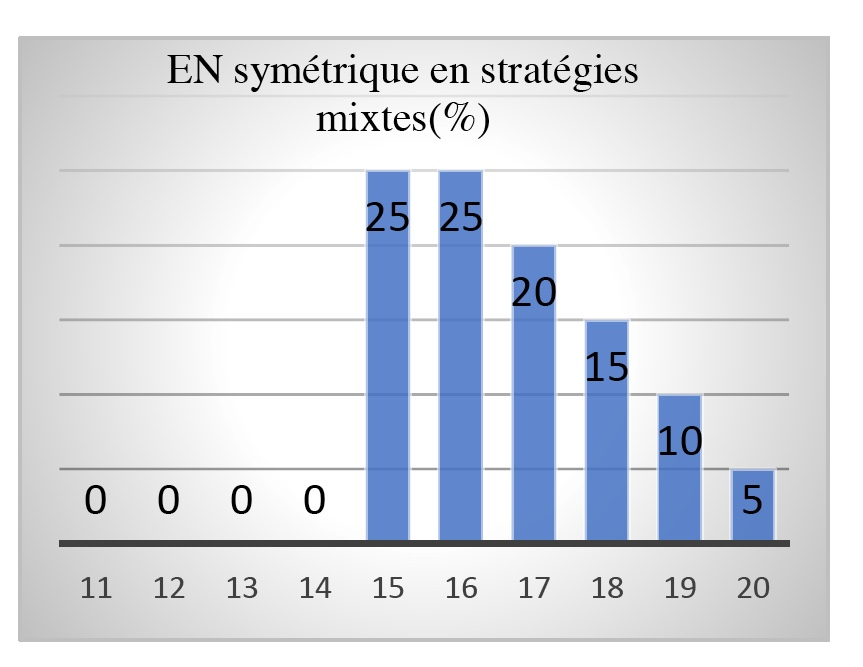
\includegraphics[height=5cm]{Articles-bons-a-composer/02_Umbhauer/02_Umbhauer_fr_Figures/02_Umbhauer_fr_figure-3.jpeg}
\end{figure}

% PROPOSITION 1

\begin{proposition}

a) Dans le jeu 11-T/bonus B, \(B \geq T > 11 + n\), n étant
l'entier naturel défini par \(\frac{n(n + 1)}{2} < B < \frac{(n + 1)(n + 2)}{2}\), la MR
stratégie mixte est donnée par~:

{\centering
$p_{i} = 0$, i de 11 à $T-n-1$, \\
$p_{T - n + i} = \frac{i + 1}{B}$, i de 0 à $n-1$,  \\
$p_{T} = 1 - \frac{n(n + 1)}{2B}$;\par}

b) Pour \(B \geq T > 11 + n\) et \(B=\frac{n(n + 1)}{2}\), les MR stratégies mixtes sont les combinaisons convexes des deux distributions suivantes :

{\centering
$p_{i} = 0$, i de 11 à $T-n-1$, \\
$p_{T - n + i} = \frac{i + 1}{B}$, i de 0 à $n-1$, \\
$p_{T} = 0$,\par}

et

{\centering
$p_{i} = 0$, i de 11 à $T-n$, \\
$p_{T - n + i} = \frac{i}{B}$, i de 1 à n;\par}

c) Le MR, z, est égal à
\(B + \frac{n(n + 1)(n + 2)}{6B}\ –\ (n + 1)\).
\end{proposition}

\begin{demonstration}
    Voir annexe~\ref{Annexe:Démonstration prop 1_Umbhauer}. \quad \blacksquare
\end{demonstration}

Le point \emph{a} est illustré dans le jeu d'Arad et Rubinstein avec \(T = B = 20\) et
\(n = 5\). Le point~\emph{b} est illustré pour \(B = T = 21\) et \(n = 6\). Deux distributions,

{\centering \(p_{i} = 0\) pour \emph{i} de 11 à 14,
$p_{15} = \frac{1}{21}, p_{16} = \frac{2}{21}, p_{17} = \frac{3}{21}, p_{18} = \frac{4}{21}$,\par}

{\centering \(p_{19} = \frac{5}{21}, p_{20} = \frac{6}{21}, p_{21} = 0\)\par}

\noindent et

{\centering $p_{i} = 0$ pour \emph{i} de 11 à 15,
$p_{16} = \frac{1}{21}, p_{17} = \frac{2}{21}, p_{18} = \frac{3}{21}, p_{19} = \frac{4}{21}$,\par} 

{\centering $p_{20} = \frac{5}{21}, p_{21} = \frac{6}{21}$,\par}

\noindent conduisent au regret minimal 50/3, et toute combinaison convexe des deux
distributions conduit également à ce regret minimal.

La proposition 1 donne lieu aux commentaires suivants.

Quand \(\frac{n(n + 1)}{2} < B,\) $p_T$
($p_20$ dans le jeu d'Arad et Rubinstein) est juste
le complément à 1 de la somme \(\sum_{i = T - n}^{T - 1}p_{i}\). Dans le
jeu d'Arad et Rubinstein, $p_T = p_{T-1} = 5/20$. Ainsi, par construction, la
probabilité de jouer le plus grand montant (qui correspond au
raisonnement de niveau-0) est inférieure ou égale à la probabilité de
jouer le montant \(T - 1\) (montant du raisonnement de niveau-1)

La proposition montre que, pour \(B > \frac{n(n + 1)}{2}\),
\emph{p\textsubscript{i}} est linéairement croissante en \emph{i}, pour
\emph{i} de \(T - n\) à \(T - 1\): $\ p_{T - n} = \frac{1}{B}$, $p_{T - 1} = \frac{n}{B}$ et $p_{i} - p_{i - 1} = 1/B$. Pour \(B = \frac{n(n + 1)}{2}\), $p_i$ est également croissante en \emph{i}, pour \emph{i} de \(T - n\) à \(T - 1\), mais $p_T$ peut être supérieure,
inférieure ou égale à $p_{T-1}$.

Ces probabilités croissantes sont en accord avec la conjecture émise en
amont : un joueur qui joue \emph{x} regrette toujours de ne pas avoir
joué \(y - 1\), \emph{y} étant le montant joué par l'adversaire, mais ce
regret décroît en \emph{x}, car \(y - 1 + B - x\) est décroissant en
\emph{x}.

La proposition 1 va au-delà du résultat de \textcite{garciapola2020}. Cet auteur a montré qu'une application itérée du MR en
stratégies pures et le raisonnement de niveau-1 conduisent à
sélectionner le même montant, 19, dans le jeu d'Arad et Rubinstein. La
proposition 1 montre que la MR stratégie mixte coïncide avec une
distribution issue d'un raisonnement de niveau-\emph{k}, du niveau-1 au
niveau-\emph{n}, à condition que chaque étape additionnelle de
raisonnement soit réalisée par un nombre plus petit d'individus. Ainsi,
dans le jeu 11-20/bonus20, les MR probabilités correspondent à la
distribution observée avec des joueurs de niveau-\emph{k}, si 25 \% des
joueurs mènent un raisonnement de niveau-1 (\emph{i.e.} jouent 19), 20~\% font
un raisonnement de niveau-2 (\emph{i.e.} jouent 18), 15~\% font un raisonnement
de niveau-3 (\emph{i.e.} jouent 17), 10~\% font un raisonnement de niveau-4
(\emph{i.e.} jouent 16) et 5~\% font un raisonnement de niveau-5 (\emph{i.e.} jouent
15). D'où, malgré que la logique du MR n'ait aucun lien avec le
raisonnement de niveau-\emph{k}, le MR conduit à un comportement
similaire dans le jeu de demande 11-\emph{T} avec bonus \emph{B}, du
moins si on suppose que le pourcentage de joueurs aptes à mener un
raisonnement de niveau-\emph{k} décroît avec \emph{k}. Comme
\emph{p\textsubscript{i} =} 0 pour \(i < T - n\), ce résultat, pour être
compatible avec le raisonnement de niveau-\emph{k}, exige que personne
ne soit capable de mener un raisonnement de profondeur supérieure ou
égale au niveau-\((n + 1)\). Toutefois, \(B \geq T > 11 + n\) et
\(B > n(n + 1)/2\) impliquent \(n \geq 5\), aussi cette limite de
profondeur de raisonnement n'est pas vraiment restrictive, car dans la
réalité les joueurs font rarement plus de quatre itérations (raisonnement de
niveau-4) (voir par exemple \textcite{crawford2013}). Plus précisément, même
s'ils sont aptes à faire plus d'itérations, ils hésitent souvent à en
faire davantage car ils craignent que les autres joueurs n'en soient pas
capables\footnote{C'est donc la théorie de l'esprit (\textit{theory of mind}),
  c'est-à-dire l'habileté à se glisser dans la façon de raisonner de
  l'autre, qui conduit souvent à stopper un raisonnement au plus tard au
  niveau-4.}.

Étant donné que \emph{n} est croissant en \emph{B}, la proposition 1
montre également que la profondeur de raisonnement des acteurs croît en
fonction du gain qu'ils peuvent obtenir, ce qui est conforme à un
résultat obtenu par \textcite{alaoui2016}. Ainsi par exemple, dans
le jeu de demande 11-20 avec un bonus \(B\) qui vaut 30 au lieu de 20,
la profondeur de raisonnement atteint 7, vu que la MR stratégie mixte
devient~: $p_{i} = 0$, $i$ de 11 à 12, $p_{13} = \frac{1}{30}$, $p_{14} = \frac{2}{30}$, $p_{15} = \frac{3}{30}$, $p_{16} = \frac{4}{30}$, $p_{17} = \frac{5}{30}$, $p_{18} = \frac{6}{30}$, $p_{19} = \frac{7}{30}$, $p_{20} = \frac{2}{30}$.


\section{MINIMAX REGRET, ÉQUILIBRE DE NASH ET GAIN ESPéRé}
\label{section:Minimax Reg équilibre}

En comparant les figures 2 et 3 on voit que les probabilités de la
figure 3, pour \emph{x} de 15 à 20, sont symétriques à celles de la
figure 2, par rapport à l'axe vertical \(x = 17,5\). On dira simplement
qu'elles sont <<inversées>>. Ce lien étonnant pousse à la réflexion car,
usuellement, il n'y a aucun lien évident entre les stratégies
sélectionnées par l'EN et le MR (voir par exemple \textcite{umbhauer2022}).
Dans les jeux 11-\emph{T}/bonus\emph{B}, il y a au contraire un lien
fort entre les deux concepts, précisé dans la proposition 2.

% PROPOSITION 2

\begin{proposition}
Dans les jeux 11-T/bonusB, avec \(B \geq T > 11 + n\), $n$ étant l'entier naturel vérifiant \(\frac{n(n + 1)}{2} < B < \frac{(n + 1)(n + 2)}{2}\), les actions
jouées à l'EN symétrique en stratégies mixtes sont les mêmes que celles
jouées dans la MR stratégie mixte. Mais les probabilités attribuées aux
montants joués sont inversées (elles sont symétriques par rapport à
l'axe vertical \(x = T - n/2\)), c'est-à-dire :
\(q_{i} = p_{2T - n - i}\) pour $i$ de \(T - n\) à $T$, où
$q_i$, respectivement $p_i$, est la
probabilité attribuée au montant $i$ par l'EN symétrique en stratégies
mixtes, respectivement la MR stratégie mixte.   
\end{proposition}

\begin{demonstration}
    Pour le montant joué $i$, le gain
\(i(1 - q_{i + 1}) + (i + B)q_{i + 1} = i + B{q\ }_{i + 1}\) doit être
égal au gain obtenu avec le montant $T$, à savoir $T$. Ainsi
\(q_{i} = \ (T - i + 1)/B\) pour $i$ de $T$ à \(T - n + 1\) et
\(q_{T - n} = 1 - \frac{n(n + 1)}{2B}\) , avec
\(\frac{n(n + 1)}{2} < B < \frac{(n + 1)(n + 2)}{2}\). Il en découle que
les montants $i$, pour \(i < T - n\), conduisent à un gain
inférieur, d'où \(q_{i} = 0\). \quad \blacksquare
\end{demonstration}

Par exemple, dans le jeu d'Arad et Rubinstein, les probabilités de l'EN
symétrique sont \(q_{i} = 0\) pour \emph{i} de 11 à
14, $q_{15} = \frac{5}{20}$, $q_{16} = \frac{5}{20}$, $q_{17} = \frac{4}{20}$, $q_{18} = \frac{3}{20}$, $q_{19} = \frac{2}{20}$ et $q_{20} = \frac{1}{20}$ (tableau~1 et figure~3).

Ainsi, alors que les MR probabilités croissent linéairement de
\(p_{T - n} = 1/B\) à \(p_{T - 1} = n/B\) (\emph{p\textsubscript{T}}
étant le complément à 1), les probabilités de l'EN symétrique
décroissent linéairement de\(\ q_{T - n + 1} = n/B\) à \(q_{T} = 1/B\ \)
($q_{T-n}$ étant le complément à 1).

\vspace{0.2cm}
Ce lien surprenant est dû à la structure des jeux étudiés. Nous
illustrons ce fait dans le jeu 11-20/bonus20. Les équations liées au MR
(1) qui sont vérifiées avec égalité sont rappelées ci-après (équations~(2)). On peut observer que ces équations sont les équations de l'EN en
stratégies mixtes, qui assurent que le joueur~2 obtienne le même gain
avec toutes ses stratégies pures dans le jeu à somme nulle de la matrice~3. Ainsi les probabilités $p_i$ du joueur~1 obtenues
par la logique du MR correspondent à la stratégie mixte du joueur~1 à
l'EN du jeu de la matrice~3.
%
\begin{align*}
19p_{15} + 18p_{16} + 17p_{17} + 16p_{18} + 15p_{19} + 14p_{20} &= z \\
0p_{15} + 19p_{16} + 18p_{17} + 17p_{18} + 16p_{19} + 15p_{20} &= z \\
21p_{15} + 0p_{16} + 19p_{17} + 18p_{18} + 17p_{19} + 16p_{20} &= z \\
22p_{15} + 21p_{16} + 0p_{17} + 19p_{18} + 18p_{19} + 17p_{20} &= z \\ \tag{2}
23p_{15} + 22p_{16} + 21p_{17} + 0p_{18} + 19p_{19} + 18p_{20} &= z \\
24p_{15} + 23p_{16} + 22p_{17} + 21p_{18} + 0p_{19} + 19p_{20} &= z \\
p_{15} + p_{16}{+ p}_{17} + p_{18} + p_{19} + p_{20} &= 1
\end{align*}

\begin{table}[h!]
\centering
Matrice 3\par
\vspace{0.2cm}
\label{matrice3}
\resizebox{.65\linewidth}{!}{
\begin{tabular}{lc | *{6}{c} |}
\multicolumn{8}{c}{P12} \tabularnewline
& \multicolumn{1}{l}{} & 15 & 16 & 17 & 18 & 19 & \multicolumn{1}{c}{20} \tabularnewline
\cline{3-8}
& 15 & (--19,19) & (0,0) & (--21,21) & (--22,22) & (--23,23) &
(--24,24) \tabularnewline
& 16 & (--18,18) & (--19,19) & (0,0) & (--21,21) & (--22,22) &
(--23,23) \tabularnewline
Pl1 & 17 & (--17,17) & (--18,18) & (--19,19) & (0,0) &
(--21,21) & (--22,22) \tabularnewline
& 18 & (--16,16) & (--17,17) & (--18,18) & (--19,19) & (0,0) &
(--21,21) \tabularnewline
& 19 & (--15,15) & (--16,16) & (--17,17) & (--18,18) & (--19,19)
& (0,0) \tabularnewline
& 20 & (--14,14) & (--15,15) & (--16,16) & (--17,17) & (--18,18)
& (--19,19) \tabularnewline
\cline{3-8}
\end{tabular}}
\end{table}

Les équations de Karush Kuhn Tucker (voir l'annexe\ref{Annexe:Démonstration prop 1_Umbhauer} dont elles sont
extraites) qui découlent du programme de minimisation deviennent les
équations~(3) (après avoir enlevé les multiplicateurs égaux à 0) :
%
\begin{align*}
19\lambda_{15} + 0\lambda_{16} + 21\lambda_{17} + 22\lambda_{18} + 23\lambda_{19} + 24\lambda_{20} + \lambda &= 0 \\
18\lambda_{15} + 19\lambda_{16} + 0\lambda_{17} + 21\lambda_{18} + 22\lambda_{19} + 23\lambda_{20} + \lambda &= 0 \\
17\lambda_{15} + 18\lambda_{16} + 19\lambda_{17} + 0\lambda_{18} + 21\lambda_{19} + 22\lambda_{20} + \lambda &= 0 \\ \tag{3}
16\lambda_{15} + 17\lambda_{16} + 18\lambda_{17} + 19\lambda_{18} + 0\lambda_{19} + 21\lambda_{20} + \lambda &= 0 \\
15\lambda_{15} + 16\lambda_{16} + 17\lambda_{17} + 18\lambda_{18} + 19\lambda_{19} + 0\lambda_{20} + \lambda &= 0 \\
14\lambda_{15} + 15\lambda_{16} + 16\lambda_{17} + 17\lambda_{18} + 18\lambda_{19} + 19\lambda_{20} + \lambda &= 0 \\
1 - \sum_{i = 15}^{20}{\lambda_{i}} &= 0
\end{align*}

Ces équations assurent que le joueur 1 réalise le même gain avec toutes
ses stratégies pures dans le jeu à somme nulle de la matrice 3. Aussi
les multiplicateurs KKT $\lambda_i$ deviennent la
stratégie mixte du joueur 2 à l'EN du jeu à somme nulle de la matrice~3.

Or il y a un lien fort entre le jeu à somme nulle de la matrice~3 et le
jeu réellement joué par les joueurs, dès lors qu'on écrit ce jeu à
l'envers, ce qui est fait dans la matrice~4.

\begin{table}[h!]
\centering
Matrice 4\par
\vspace{0.2cm}
\label{matrice4}
\resizebox{.65\linewidth}{!}{
\begin{tabular}{lc | *{6}{r} | }
\multicolumn{8}{c}{P12} \tabularnewline
& \multicolumn{1}{l}{} & 20 & 19 & 18 & 17 & 16 & \multicolumn{1}{c}{15} \tabularnewline
\cline{3-8}
& 20 & (20,20) & (20,39) & (20,18) & (20,17) & (20,16) & (20,15) \tabularnewline
& 19 & (39,20) & (19,19) & (19,38) & (19,17) & (19,16) & (19,15) \tabularnewline
Pl1 & 18 & (18,20) & (38,19) & (18,18) & (18,37) & (18,16) & (18,15) \tabularnewline
& 17 & (17,20) & (17,19) & (37,18) & (17,17) & (17,36) & (17,15) \tabularnewline
& 16 & (16,20) & (16,19) & (16,18) & (36,17) & (16,16) & (16,35) \tabularnewline
& 15 & (15,20) & (15,19) & (15,18) & (15,17) & (35,16) & (15,15) \tabularnewline
\cline{3-8}
\end{tabular}}
\end{table}

En effet, égaliser les gains du joueur 2 dans deux colonnes adjacentes
de la matrice 4 conduit exactement aux mêmes calculs qu'égaliser les
gains des mêmes colonnes de la matrice 3, car ces égalisations
exploitent les différences 1 et 19 qui sont présentes dans les deux
matrices exactement aux mêmes emplacements.

Par exemple, égaliser les gains du joueur 2 dans les deux premières
colonnes des deux matrices conduit aux équations~:
\begin{equation*}
\begin{split}
  20p_{20} + 20p_{19} + 20p_{18} + 20p_{17} + 20p_{16} + 20p_{15} = 39p_{20} + 19p_{19} + 19p_{18}\\ + 19p_{17} + 19p_{16} + 19p_{15}  
\end{split}
\end{equation*}

\noindent \text{pour la matrice 4 (on note \emph{p\textsubscript{i}} la probabilité du
joueur 1 de jouer \emph{i})} et
\begin{equation*}
\begin{split}
    19p_{15} + 18p_{16} + 17p_{17} + 16p_{18} + 15p_{19} + 14p_{20} = 0p_{15} + 19p_{16} + 18p_{17}\\ + 17p_{18} + 16p_{19} + 15p_{20}
\end{split}
\end{equation*}

\noindent \text{pour la matrice 3.}

Ces équations conduisent à \(p_{20} = \frac{1}{20}\) pour la matrice 4
et \(p_{15} = \frac{1}{20}\) pour la matrice 3. Et c'est ainsi qu'on
obtient les probabilités inversées.

Ajoutons quelques remarques au sujet des gains.

On peut commencer par observer que le MR, si les deux joueurs jouent
leur MR stratégie mixte, conduit au gain espéré 21.5 dans le jeu d'Arad
et Rubinstein, soit un gain plus élevé que le gain espéré 20 de l'EN
symétrique.

Ce résultat se généralise à tout jeu \(11 - T/bonusB\), où
\(B \geq T > n + 11\), \emph{n} étant défini par
\(\frac{n(n + 1)}{2} < B < \frac{(n + 1)(n + 2)}{2}\) (partie \emph{a}
de la proposition 3).

Toutefois minimiser les regrets n'est adapté que dans un contexte à
forte incertitude stratégique où l'adversaire est susceptible de jouer
n'importe quelle stratégie. Aussi un joueur jouant la MR stratégie mixte
n'est pas nécessairement confronté à un adversaire jouant également
cette stratégie. Il est donc plus pertinent de calculer le gain obtenu
par un joueur jouant la MR stratégie mixte face à tout montant
potentiellement joué par son adversaire. Ce calcul donne lieu à la
partie (\emph{b}) de la proposition 3.

% PROPOSITION 3

\begin{proposition}

a) Dans tout jeu 11-T/bonusB, avec \(B \geq T > n + 11\), n
étant l'entier naturel vérifiant \(\frac{n(n + 1)}{2} < B < \frac{(n + 1)(n + 2)}{2}\), le gain espéré avec le MR, lorsque les deux joueurs jouent leur MR stratégie
mixte, vaut \(T + n - \frac{n(n + 1)(n + 2)}{3B}\). Ce gain est
entre \(T + \frac{n - 4}{3}\) et \(T + \frac{n}{3}\), et
est donc strictement plus grand que T, vu que n est plus grand que 4. Il
est donc plus grand que le gain espéré de l'EN symétrique, qui, par
construction, est toujours égal à T, quel que soit n. \par
b) On suppose maintenant que l'adversaire joue le montant~y. Alors un joueur qui joue la MR stratégie mixte obtient un paiement moyen égal à~:

{\centering
\(y - 1 + B - z = y + n - \frac{n(n + 1)(n + 2)}{6B}\) si \(y \geq \ T - n\),\\
\(T - \frac{n(n + 1)(n + 2)}{6B}\) si \(y < T - n\).\par}

Ainsi le gain le plus bas auquel mène la MR stratégie mixte est
entre \(T - (n + 2)/3\) et \(T - n/3\) et le gain le plus
élevé est \(T + n - \frac{n(n + 1)(n + 2)}{6B}\), qui est entre
\(T + 2(n - 1)/3\) et \(T + 2n/3\ \). La MR stratégie mixte
conduit à un gain supérieur à celui de l'EN symétrique dès que
\(y > T - n + \frac{n(n + 1)(n + 2)}{6B}\), \(T - n + \frac{n(n + 1)(n + 2)}{6B}\)
étant entre \(T - 2n/3\) et \(T - 2(n - 1)/3\).    
\end{proposition}

\begin{demonstration}
    Voir l'annexe~\ref{Annexe:Démonstration prop 3_Umbhauer}. \quad \blacksquare
\end{demonstration}

Par exemple (partie \emph{a}), pour \(T = 100,\ B = 100,\ n = 13\), le
paiement espéré quand les deux joueurs jouent la MR stratégie mixte est
103,9 au lieu de 100 (paiement espéré dans l'EN symétrique). Toutefois,
si on reste dans l'esprit du jeu d'Arad et Rubinstein et qu'on garde
\(B = T\), alors la différence entre les gains associés à l'EN et à la
MR stratégie mixte, comparée à \emph{T}, reste faible. En effet, comme
\(n(n + 1)/2 < B\), on a \(n/3 < \sqrt{2B}/3\) et, vu que le gain espéré
avec le MR est plus faible que \(T + n/3\), il est plus faible que
\(T + \sqrt{2T}/3\). Aussi la différence entre les deux gains est certes
croissante en \emph{T}, mais la différence relative par rapport à
\emph{T}, \(\frac{\sqrt{2T}}{3T},\) est décroissante en \emph{T}. Ce
résultat change quand \emph{B} peut être nettement plus grand que
\emph{T} (avec \(T > 11 + n\)). Dans ce cas, le gain additionnel peut
avoisiner \((T - 11)/3\), un montant qui peut être conséquent.

La partie~\emph{b} peut être illustrée dans le jeu d'Arad et Rubinstein
(tableau 2).

\begin{table}[h!]
\caption{Gain moyen de la MR stratégie mixte dans le jeu
  11-20/bonus20 en fonction du montant choisi par l'adversaire}\label{tabl2}
\centering
\resizebox{\linewidth}{!}{
\begin{tabular}{l*{10}{D{6mm}}}
\toprule
Montant demandé \par par l'adversaire & \centering 11 & \centering 12 & \centering 13 & \centering 14 & \centering 15 & \centering 16 & \centering 17 & \centering 18 & \centering 19 & \centering 20 \tabularnewline
\midrule
MR paiement & 18,25 & 18,25 & 18,25 & 18,25 & 18,25 & 19,25 & 20,25 &
21,25 & 22,25 & 23,25 \tabularnewline
\bottomrule
\end{tabular}}
\end{table}

Ainsi, même si l'adversaire joue les nombres -- peu fréquemment joués~--
de 11 à 15, le gain du joueur est plutôt grand, et le fait que ce gain
soit plus faible que le gain 20 de l'EN en stratégies mixtes doit être
contrebalancé par le fait qu'il est plus grand que 20 lorsque
l'adversaire joue les nombres -- plus fréquemment joués~-- de 17 à 20.

Si \(T = B = 100\), \(n = 13\)\emph{,} le tableau de gains devient le
tableau 3:

\begin{table}[h!]
\caption{Gain moyen de la MR stratégie mixte dans le jeu
  11-100/bonus100 en fonction du montant choisi par l'adversaire}\label{tabl3}
\centering
\resizebox{\linewidth}{!}{
\begin{tabular}{l*{14}{D{6mm}}}
\toprule
 Montant demandé par l'adversaire & Toute valeur $\leq$~87 & 88 & 89 & 90 & 91 & 92 & 93 & 94 & 95 & 96 & 97 & 98 & 99 & 100 \tabularnewline
\midrule
MR paiement & 95,45 & 96,45 & 97,45 & 98,45 & 99,45 & 100,45 & 101,45 &
102,45 & 103,45 & 104,45 & 105,45 & 106,45 & 107,45 & 108,45 \tabularnewline
\bottomrule
\end{tabular}}
\end{table}

À nouveau les paiements sont plutôt attractifs. Ils sont plus faibles
que le gain 100 de l'EN symétrique quand l'adversaire joue des nombres
inférieurs à 92 (mais restent élevés, 95,45 au moins au lieu de 100)
mais ils sont plus grands que 100 (et croissent jusqu'à 108,45) quand
l'adversaire jouent des nombres supérieurs ou égaux à 92.

Plus généralement, quand \emph{n} devient grand, alors le paiement
minimal auquel peut conduire le MR, proche de \(T - n/3\), peut certes
devenir faible en comparaison du paiement \emph{T} de l'EN (surtout si
\emph{B} est beaucoup plus grand que \emph{T}). Mais, dans le même
temps, le montant minimal \emph{y} de l'adversaire, autour de
\(T - 2n/3\), à partir duquel le MR conduit à un gain plus élevé que le
gain de l'EN, devient beaucoup plus petit. Aussi, à condition que
l'adversaire joue des nombres plutôt élevés (ce qui est usuellement
observé dans les expériences), la MR stratégie mixte conduit à des gains
plus élevés que l'EN.

\section{COMMENTAIRES SUR LES MINIMAX REGRETS, \\ VARIANTES DU JEU DE DEMANDE 11-20 \\ AVEC BONUS 20 ET AVERSION AU RISQUE}
\label{section:Commentaires sur MR}

\textcite{arad2012} ont observé que dans leur jeu
11-20/bonus20, seul un petit nombre de leurs étudiants, moins de 20~\%,
faisaient plus de trois itérations, et ce malgré qu'une itération
supplémentaire --~à savoir passer du montant \emph{x} de niveau-\emph{k}
au montant $x-1$ de niveau-\emph{k}+1~-- ne requiert que très peu
de compétences cognitives. Aussi ils ont essayé de stimuler davantage
d'itérations en renforçant la légitimité du montant 20 comme point
d'ancrage des itérations.

Pour ce faire ils ont introduit une version cyclique, qui ne diffère de
la version de base que par le fait qu'un joueur qui joue 20 obtient le
bonus 20 si son adversaire joue 11. Le choix de 20 est ainsi encore plus
attractif que dans la version initiale du jeu~: 20 devient donc encore
plus spontanément la stratégie naturelle de niveau-0. En ce qui concerne
les étudiants de Strasbourg, il est probable que ce changement aurait
poussé certains des étudiants jouant 13, 14 et 15 dans la version
initiale du jeu d'Arad et Rubinstein à choisir 18, 19 et 20. En effet la
moitié de ces étudiants justifiaient le jeu de 13, 14 et 15 par un
raisonnement de niveau-\emph{k} débutant par 15 ou 16 (donc fixaient 15
ou 16 comme l'action de niveau-0). Toutefois, renforcer 20 en tant que
point d'ancrage du raisonnement de niveau-\emph{k} n'a pas augmenté la
profondeur de raisonnement\footnote{Cela est peut-être dû au fait que
  faire plus d'itérations ne conduit pas à un gain additionnel ; dans
  les faits, le paiement additionnel de 20 dans cette version cyclique
  n'est obtenu qu'en jouant 20 lorsque l'adversaire joue 11, ce qui
  nécessite 10 itérations, un nombre généralement non atteint (plus
  exactement, un joueur doit espérer que l'adversaire joue 11, donc mène
  un raisonnement de niveau-9, ce qu'il ne fait généralement pas).}. Au
contraire, la version cyclique a augmenté le nombre de joueurs de
niveau-1, comme on peut le voir dans le tableau~4. L'EN symétrique reste
lui inchangé ainsi que le paiement espéré 20 à cet équilibre.

Étudions comment évolue la MR stratégie mixte dans cette nouvelle
version du jeu.

En fait, pour établir la MR stratégie mixte dans ce nouveau jeu, il
suffit de changer la première contrainte dans (1). Cette contrainte
devient~:
\[29p_{11} + 28p_{12} + 27p_{13} + 26p_{14} + 25p_{15} + 24p_{16} + 23p_{17} + 22p_{18} + 21p_{19} + 0p_{20} \leq z.\]
Si on associe cette contrainte à la dernière, on obtient la relation
additionnelle \(1 + 20p_{19} = 20p_{20}\), ce qui explique une
distribution de probabilités strictement croissante de 15 à 20. Il
s'ensuit que les probabilités dans la version cyclique sont pratiquement
les mêmes que dans la version initiale du jeu, excepté qu'elles sont un
peu plus faibles pour les montants de 15 à 19, et que la probabilité
attribuée à 20 est plus élevée (29,17~\% au lieu de 25~\%). Cette
distribution, même si on se limite aux nombres de 16 à 20, est
différente de la distribution obtenue par AR dans ce nouveau jeu (la
valeur \emph{p} du test du khi-deux vaut 0,015), mais les deux
distributions partagent un point commun important : elles sont
strictement croissantes de 15 à 19\footnote{De façon assez surprenante,
  la distribution d'AR (72~joueurs) dans la version cyclique, lorsqu'on
  se limite aux montants de 16 à 20, n'est pas significativement
  différente de la distribution de Strasbourg pour la version initiale
  -non cyclique- du jeu (test du khi-deux, \(p = 0,15\)). En quelque
  sorte, cela peut signifier que les étudiants de Strasbourg ont
  spontanément fait de 20 un point d'ancrage important.}. De plus, la MR
stratégie mixte conduit à des gains élevés, peu importe le montant
choisi par l'adversaire (voir tableau 4).

\begin{table}[h!]
\caption{Distribution expérimentale d'AR, minimax regret en
  stratégies mixtes, équilibre de Nash symétrique et paiement moyen du
  minimax regret dans la version cyclique d'AR}\label{tabl4}
\centering
\resizebox{\linewidth}{!}{
\begin{tabular}{l*{10}{D{6mm}}}
\toprule
Montant demandé dans la version cylique & \centering 11 & \centering 12 & \centering 13 & \centering 14 & \centering 15 & \centering 16 & \centering 17 & \centering 18 & \centering 19 & \centering 20 \tabularnewline
\midrule
Expérience d'AR (\%) & 1 & 1 & 0 & 1 & 0 & 4 & 10 & 22 & 47 & 13 \tabularnewline
MR strategie (\%) & 0 & 0 & 0 & 0 & 4,17 & 9,17 & 14,17 & 19,17 & 24,17 &
29,17 \tabularnewline
EN symétrique (\%) & 0 & 0 & 0 & 0 & 25 & 25 & 20 & 15 & 10 & 5 \tabularnewline
MR paiement en fonction du montant demandé par l'adversaire & 24,21 & 18,375 &
18,375 & 18,375 & 18,375 & 19,21 & 20,21 & 21,21 & 22,21 & 23,21 \tabularnewline
\bottomrule
\end{tabular}}
\end{table}

Plus généralement, dans toutes les variantes de leur jeu 11-20/bonus20
étudiées dans AR [2012], Arad et Rubinstein ont rarement observé des
étudiants effectuant plus de trois itérations. Étant donné le peu de
ressources cognitives nécessaires pour réaliser plus de 3 itérations
dans ces jeux, ils en ont déduit qu'il devait exister un seuil
d'itérations \emph{k} supérieur, que les acteurs ne franchissent pas ou
ne souhaitent pas franchir. Nous arguons toutefois dans cet article que
le raisonnement de niveau-\emph{k} n'est pas seul à l'œuvre dans les
jeux étudiés : il doit au moins partiellement être contrebalancé par la
façon dont les individus gèrent les regrets, le regret de ne pas obtenir
le bonus et le regret de ne pas avoir le gain certain 20. Un simple
regard aux explications apportées par les étudiants dans l'expérience en
classe de Strasbourg montre qu'ils parlent de regrets. Par exemple,
lorsqu'ils jouent 19, ils disent qu'« au plus ils regrettent l'unité
additionnelle qu'il auraient pu avoir en jouant 20, mais qu'en échange
ils ont l'opportunité de gagner 39 si l'adversaire joue 20\footnote{Le
  fait qui importe dans cette phrase est qu'elle ne contient pas le
  terme~distribution de probabilités. Le jeu de 19 ne s'explique pas par
  le fait que 19 est la meilleure réponse (comportement de niveau-1)
  dans un environnement perturbé où les joueurs de niveau-0 joueraient
  20 avec une forte probabilité mais inférieure à 1 (ce qui conduirait à
  comparer les stratégies 19 et 20, et donc des différences de $-1$ et
  20). Le comportement exprimé dans cette phrase est en accord avec le
  MR car le joueur joue 19 quelle que soit la demande (ou distribution
  de probabilités sur les demandes) de l'adversaire. Il joue 19 car au
  plus il regrette 1 en comparaison avec le gain certain 20 (il ne
  regrette donc pas un manque de prudence) et il ne regrette pas le
  potentiel bonus 20 (vu qu'il garde l'opportunité de l'obtenir).}~». De
même, quand ils jouent 16, 17, 18 ils ajoutent souvent au raisonnement
de niveau-\emph{k} (quand ils le font) l'observation qu'au plus ils perdent 4,
3 ou 2 par comparaison au jeu de 20. Ainsi ils ne calculent pas les
regrets en comparant les paiements des meilleures réponses aux paiements
obtenus, mais en comparant le gain sûr \emph{x} qu'ils obtiennent en
jouant \emph{x}, avec le gain sûr de 20 qu'ils pourraient obtenir en
jouant 20. Or le regret quand l'adversaire joue \emph{y}
\(( \neq x + 1)\), tel qu'il est défini par le concept de MR, est
\(B + y - 1 - x\), et peut donc s'écrire \((20 - x) + B + y - 1 - 20\).
Aussi comparer le regret associé à deux stratégies \emph{x} et $x'$
quand l'adversaire joue \emph{y} (\(y \neq x + 1\) et
\(y \neq \ x’ + 1\)), revient à comparer \(20 - x\) et \(20 - x'\), les
montants que les étudiants prennent en compte quand ils parlent de
regrets. En fait, dans l'expérience en classe de Strasbourg, si peu
d'étudiants vont au-delà de trois itérations, ce qui les conduirait à jouer
un nombre \emph{x} inférieur à 17, cela tient au fait que ces regrets
deviennent larges quand \emph{x} est loin de 20.

Deux expériences qui montrent que le MR et le raisonnement de
niveau-\emph{k} sont tous deux présents dans le jeu 11-20/bonus20 sont
celles proposées par \textcite{goeree2018} (GLZ par la suite), qui
sont deux variantes du jeu d'Arad et Rubinstein. Dans ces variantes, GLZ
ont changé l'ordre des entiers naturels joués comme suit~: les joueurs
sont face à 10 boîtes alignées, numérotées de 11 à 20 dans le désordre.
Chaque joueur sélectionne une boîte et obtient le montant qui correspond
au numéro de la boîte. Et il obtient un bonus de 20 si la boîte qu'il
choisit est adjacente et à gauche de la boîte choisie par l'autre
joueur.

GLZ ont proposé les deux alignements de boîtes suivants (tableau 5):

\begin{table}[h!]
\caption{Les deux alignements proposés par Goeree, Louis et Zang [2018]}
\label{tab5}
\centering
\resizebox{\linewidth}{!}{
\begin{tabular}{l*{20}{c}}
\toprule
1\textsuperscript{er} alignement & & \cellcolor{gray!50}14 & & \cellcolor{gray!50}13 & & \cellcolor{gray!50}12 & & \cellcolor{gray!50}11 & & \cellcolor{gray!50}19 & & \cellcolor{gray!50}18 & & \cellcolor{gray!50}17 & & \cellcolor{gray!50}16 & & \cellcolor{gray!50}15 & & \cellcolor{gray!50}20 \tabularnewline
\midrule
% & & & & & & & & & & & & & & & & & & & & \tabularnewline
\midrule
2\textsuperscript{e} alignement & & \cellcolor{gray!50}19 & & \cellcolor{gray!50}18 & & \cellcolor{gray!50}17 & & \cellcolor{gray!50}16 & & \cellcolor{gray!50}15 & &
\cellcolor{gray!50}14 & & \cellcolor{gray!50}13 & & \cellcolor{gray!50}12 & & \cellcolor{gray!50}11 & & \cellcolor{gray!50}20 \tabularnewline % attention, l'espace entre la couleur et le chiffre est prise en compte, ce qui décale le nombre dans la boîte grise. C'est un bug, en attendant il faut "coller" la commande au nombre.
\bottomrule
\end{tabular}}
\end{table}

Ces deux alignements ont en commun le fait que seul le choix de (la
boîte) 20 ne peut jamais conduire au bonus et que le choix de toute
autre boîte fait obtenir le bonus dans un seul cas. Ainsi, dans le
1\textsuperscript{er} alignement, choisir (la boîte)15 conduit au bonus
quand l'adversaire choisit (la boîte) 20, 16 conduit au bonus quand
l'adversaire joue 15 et ainsi de suite. Le choix de 20, puisqu'il
correspond à la boîte la plus à droite et qu'il conduit au plus grand
gain certain sans aucun raisonnement est à nouveau la stratégie
naturelle de niveau-0 dans les deux alignements. Ainsi l'esprit du jeu
d'Arad et Rubinstein est respecté dans les deux jeux. Mais les
distributions expérimentales de GLZ obtenues pour les deux alignements
ne ressemblent pas à celles obtenues pour le jeu 11-20/bonus20. Elles
sont données en figure 4a et figure 4b.

\begin{figure}[h]
  \centering
  \caption{Distribution expérimentale de GLZ}
  \subfloat[Avec le 1\textsuperscript{er} alignement de boîtes]{%
    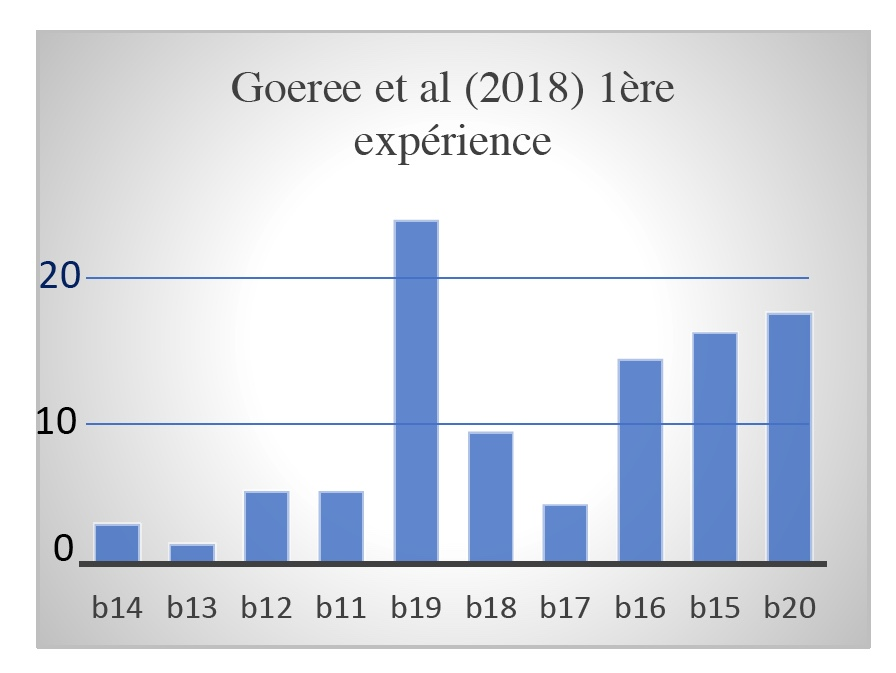
\includegraphics[height=5cm]{Articles-bons-a-composer/02_Umbhauer/02_Umbhauer_fr_Figures/02_Umbhauer_fr_figure-4a.jpeg}
    \label{fig:subfig1}%
  }
  \quad
  \subfloat[Avec le 2\textsuperscript{e} alignement de boîtes]{%
    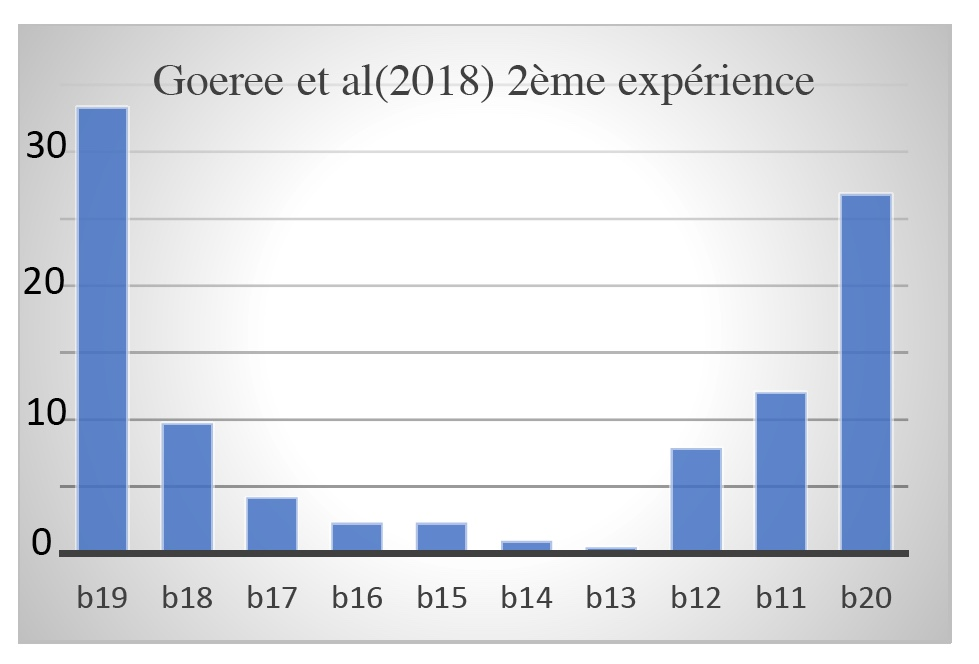
\includegraphics[height=5cm]{Articles-bons-a-composer/02_Umbhauer/02_Umbhauer_fr_Figures/02_Umbhauer_fr_figure-4b.jpeg}
    \label{fig:subfig2}%
  }
    \label{fig:mainfig}
\end{figure}

Dans les deux expériences il y a des joueurs qui ont un comportement
compatible avec un raisonnement de niveau-0, de niveau-1 et de niveau-2.
Dans la première expérience, les pourcentages de joueurs choisissant les
nombres 20, 15 et 16 sont plus grands que les pourcentages de joueurs
optant pour tout autre nombre, excepté 19. Dans la deuxième expérience,
les pourcentages associés aux nombres 20, 11 et 12 sont plus grands que
ceux associés aux autres nombres, excepté 19 et 18. Mais parallèlement,
tout d'abord, il y a très peu de joueurs de niveau-3 dans les deux
expériences et la somme des pourcentages de joueurs de niveaux 1, 2 et 3
est plutôt basse. Elle est inférieure à 35~\% dans la
1\iere{}~expérience, et plus faible que 21~\% dans la
2\ieme{}~expérience, d'où ces pourcentages sont très
différents de ceux obtenus pour le jeu 11-20/bonus20 (74~\% dans AR, 83~\%
dans LR, 60,4~\% dans l'expérience en classe de Strasbourg). Ensuite, 19
est le montant le plus souvent joué quel que soit son rang dans le
raisonnement de niveau-\emph{k} (19 est le montant de niveau-5 dans la
1\iere{}~expérience et le montant de niveau-9 dans la
2\ieme{}~expérience). Et même 18 est souvent joué dans les
deux expériences quel que soit son rang dans le raisonnement de
niveau-\emph{k}. Enfin, 20 est bien plus souvent joué que dans le jeu
11-20/bonus20 dans les deux expériences et plus particulièrement la
deuxième (27~\%). Ainsi, clairement, le fait que les grands nombres
conduisent à des gains certains élevés, et le fait que 19 assure le
2\ieme{} meilleur gain plus une opportunité d'obtenir le
bonus, jouent un rôle essentiel.

GLZ ont montré comment la connaissance commune d'un bruit dans le
comportement pouvait conduire à un comportement plus proche des données
expérimentales. Le MR permet aussi ce rapprochement. Il est intéressant
d'observer que la MR stratégie mixte est parfaitement insensible à
l'ordre des boîtes (à condition que 20 soit la boîte la plus à droite) :
ainsi le MR conduit à la même stratégie dans les deux jeux de GLZ et
dans le jeu 11-20/bonus20. Cela tient au fait que la structure des
regrets est la même dans les trois jeux. Par exemple, le fait que 19
conduise au gain 39 quand l'adversaire joue 18 (dans les deux
expériences de GLZ) conduit à une colonne de regrets qui est la même que
celle obtenue quand l'adversaire joue 20 dans le jeu d'Arad et
Rubinstein. Le fait que 15 mène à un gain de 35 quand l'adversaire joue
19 (1\iere{}~expérience) et 14 (2\ieme{}~expérience) conduit à une colonne de regrets qui est la même que celle
obtenue quand l'adversaire joue 16 dans le jeu d'Arad et Rubinstein. Et
ainsi de suite. Aussi minimiser les regrets conduit aux mêmes
contraintes dans les trois jeux (seul l'ordre des contraintes change).
Il découle que le MR conduit à la distribution de probabilités de la
figure 2. Certes, dans les jeux de GLZ, la MR stratégie mixte ne
ressemble plus à la distribution obtenue avec des joueurs de
niveau-\emph{k} (quand le pourcentage de joueurs de niveau-\emph{k}
décroît avec \emph{k}). Mais le MR est en accord avec les deux résultats
essentiels obtenus dans les expériences de GLZ. Premièrement, le MR
assigne la probabilité 0,25 à 19, une probabilité comparable aux
pourcentages obtenus dans les expériences de GLZ (24~\% dans la première
expérience, 33~\% dans la seconde expérience). Deuxièmement, la somme des
probabilités assignées à 18, 19 et 20 par le MR est 0,7, un nombre qui
est du même ordre que la somme des pourcentages de jeu de 18, 19 et 20
dans les expériences de GLZ (51~\% dans la première expérience, 70~\% dans
la seconde).

Ajoutons quelques mots au sujet de l'EN et de l'aversion au risque. Le
MR exploite le côté prudent des montants élevés (notamment 19) et le
regret associé à la non-obtention du bonus. \textcite{li2018}
exploitent également le côté prudent de 19 et 20 ; ils travaillent avec
l'EN et montrent que l'EN peut également être proche d'une distribution
expérimentale, à condition de prendre en compte l'aversion au risque.
Ils montrent notamment que la fonction d'utilité concave
\(1 - e^{- 0,15x}\), où \emph{x} est le montant choisi, conduit à un EN
qui correspond mieux à leurs données expérimentales, car cet équilibre
augmente notamment les probabilités attribuées à 18, 19 et 20. C'est
exact, mais cela ne veut pas dire que l'EN en stratégies mixtes est bien
adapté pour expliquer le comportement des joueurs. Ainsi il importe
d'observer que la fonction d'utilité \(1 - e^{- ax}\), avec \(a > 0\),
donne lieu à un EN qui se comporte comme l'EN usuel (neutre au risque) :
quand les montants joués à l'équilibre vont de \emph{x} à 20, la
probabilité attribuée à chaque nombre de \(x + 1\) à 20 décroît en ce
nombre, la probabilité de jouer \emph{x} étant le complément à 1. D'un
point de vue comportemental, il est plutôt étrange de voir \(x + 1\ \)
joué avec la plus forte probabilité alors que \(x - 1\ \)est joué avec
la probabilité~0. En fait, par définition, dans un EN en stratégies
mixtes, les probabilités d'un joueur ont pour unique fonction de
stabiliser (optimiser) le comportement des autres joueurs. Ainsi, dans
le jeu d'Arad et Rubinstein, elles ont pour seul rôle d'assurer le gain
20 à l'adversaire quel que soit le montant qu'il joue avec une
probabilité positive : cela n'est usuellement pas l'objectif des joueurs
dans les expériences.

\section{CONCLUSION}
\label{section:Conclusion Umbhauer_fr}

Le jeu 11-20/bonus20 d'Arad et Rubinstein est un jeu fort riche qui
suscite un comportement plus nuancé que le raisonnement de
niveau-\emph{k}.

Certes, les raisonnements de niveau-\emph{k}, et plus spécifiquement de
niveau-1, niveau-2 et niveau-3, sont observés dans les expériences. Dans
l'expérience en classe menée à Strasbourg, le raisonnement de
niveau-\emph{k} prédomine clairement chez les nombreux étudiants
(32,4~\%) qui jouent 17 et 18. La plupart des étudiants jouant 18 font
exclusivement un raisonnement de niveau-2, et 60~\% des étudiants jouant
17 font exclusivement un raisonnement de niveau-3. Près de la moitié des
5,8~\% d'étudiants jouant 16 font même un raisonnement de niveau-4.

Mais la minimisation des regrets joue également un rôle important. Nous
insistons ici sur une différence notable entre le jeu 11-20/bonus20
et le jeu de devinette, qui est le jeu le plus utilisé pour étudier le
raisonnement de niveau-\emph{k}. Dans un jeu de devinette, pour être le
gagnant (pour gagner 1), un joueur doit faire une itération
additionnelle par rapport aux autres joueurs, faute de quoi il gagne 0,
le gain des perdants. Ce n'est clairement pas le cas dans le jeu
d'Arad et Rubinstein où un joueur peut gagner une somme importante sans
faire la moindre anticipation. Jouer 20 conduit au gain élevé et certain
20, quel que soit l'adversaire rencontré. Dans l'expérience en classe,
le calcul du paiement moyen de chaque stratégie confrontée à toutes les
autres stratégies jouées montre que 20 procure le 4\ieme
meilleur gain (voir la figure~5). Et 19, le montant de niveau-1, conduit
au 2\ieme{} meilleur gain. Cela explique amplement
pourquoi les étudiants à Strasbourg qui jouent 19 et 20 généralement ne
justifient pas leur comportement par un raisonnement de niveau-\emph{k}.
Comme dit précédemment, la principale justification du jeu de 19 est en
accord avec le MR~: «~En jouant 19, je gagne 19 de manière certaine, ce
qui n'est pas loin de 20, et je garde l'opportunité de gagner 39 en
rencontrant un étudiant qui joue 20~».

\begin{figure}[h]
    \centering
    \caption{Paiement moyen associé à chaque montant demandé}
    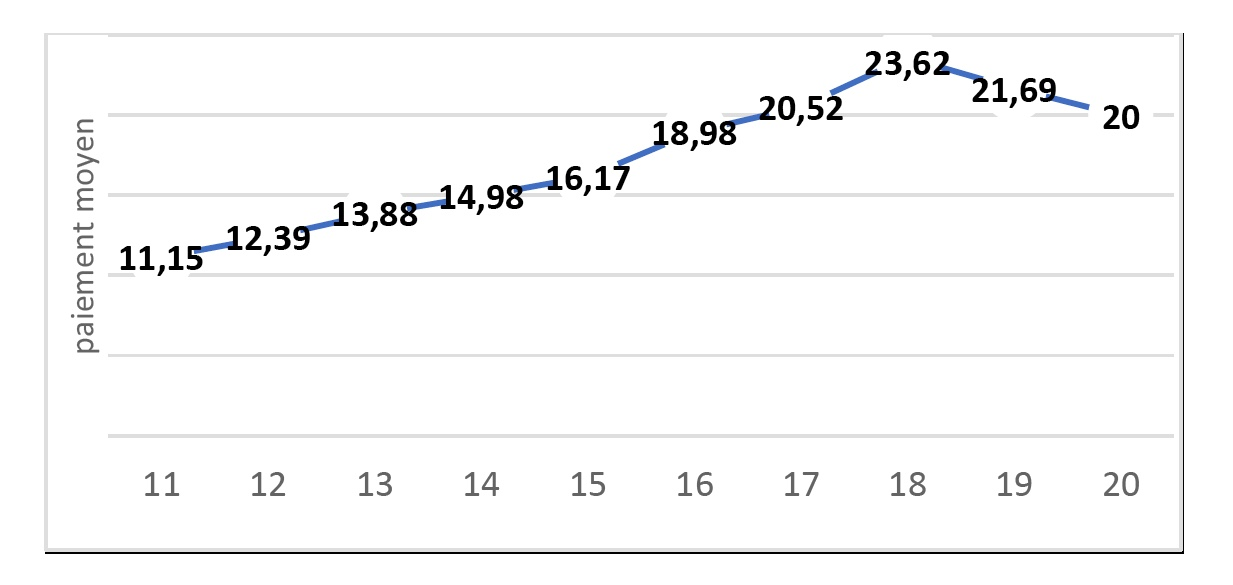
\includegraphics[height=5cm]{Articles-bons-a-composer/02_Umbhauer/02_Umbhauer_fr_Figures/02_Umbhauer_fr_figure-5.jpeg}
\end{figure}

Pour clore l'article, on peut mettre en lumière certaines particularités
de l'expérience en classe de Strasbourg, potentiellement liées au fait
que les étudiants disposaient de la matrice de la forme normale du jeu.
Cette matrice les a aidés à comparer leur gain avec celui de
l'adversaire dans chacune des configurations possibles et cela peut
expliquer certains comportements qui n'ont pas de lien, ni avec le
raisonnement de niveau-\emph{k}, ni avec la minimisation des regrets.

Ainsi beaucoup d'étudiants à Strasbourg, 8,3~\% d'entre eux, ont joué 11,
uniquement pour ne pas offrir à l'adversaire l'opportunité d'obtenir le
bonus. Il est bien connu que la peur de ne pas recevoir quelque chose
(ici le bonus) suscite l'envie que les autres ne l'obtiennent pas non
plus. Et jouer 11 est l'unique moyen d'empêcher l'adversaire d'obtenir
le bonus. En jouant 11, certains étudiants ont aussi cherché à minimiser
la différence potentielle de gains (à leur désavantage) entre les deux
joueurs. En effet, quand on joue 11, l'adversaire peut au plus gagner 9~unités de plus, alors qu'il peut gagner 19~unités supplémentaires si on
joue un montant différent de 11.

De façon moins extrême (et radicalement opposée), les étudiants qui ont
joué 19, respectivement 20, ont parfois justifié leur jeu en faisant
observer qu'ils gagnent plus que leur adversaire dans toutes les
situations, excepté une (quand l'adversaire joue 18, respectivement 19).
En effet, un étudiant qui joue 19 gagne plus que son adversaire si ce
dernier joue 20 ou un montant de 11 à 17 ; il ne gagne moins que lui que
si ce dernier joue 18. Ainsi il a un meilleur gain que son adversaire
dans 8 parmi les 10 configurations possibles. Il en va de même pour un
étudiant qui joue 20. Et on peut observer, de 18 à 11, que plus le
montant joué par un joueur est bas, moins les
configurations dans lesquelles il gagne plus que son adversaire sont nombreuses : en
jouant 18, il a un meilleur gain dans sept configurations, en jouant 11, il
n'a un meilleur gain que dans une configuration. Le fait que beaucoup
d'étudiants accordent plus d'importance à la différence de gains qu'au
gain obtenu est sûrement lié à leur vie de tous les jours. Beaucoup
d'entre eux~passent des concours où le seul objectif de chaque
participant est d'obtenir de meilleurs résultats que les autres
participants.

En somme, malgré sa simplicité, le jeu 11-20/bonus20 d'Arad et Rubinstein génère des façons contrastées de jouer~: il s'avère plus riche que ne l'anticipaient ses créateurs.

\printbibliography

\clearpage

\begin{appendices}
  
\section{Démonstration de la proposition 1}
\label{Annexe:Démonstration prop 1_Umbhauer}

\emph{a}) On résout :
\[
\min_{z\ p_{11}\ldots p_{T}}z
\]
s.c.
\[
\sum_{i = 11}^{T}{(T - i)p_{i}} \leq z
\]
\[
0p_{11} + \sum_{i = 12}^{T}{(B + 11 - i)p_{i} \leq z} \tag{A1}
\]
\[
\sum_{i = 11}^{j - 2}{(B + j - 1 - i)p_{i} + 0p_{j - 1} + \sum_{i = j}^{T}{(B + j - 1 - i)p_{i} \leq z}} \quad \text{ \emph{j} de 13 à } T
\]
\[
\sum_{i = 11}^{T}{p_{i} = 1}
\]
\[
p_{i} \geq 0 \quad \text{\emph{i} de 11 à \emph{T}}.
\]

On suppose que seuls les \emph{p\textsubscript{i}}, tels que
\(i \geq \ T - n\), sont strictement positifs, avec \emph{n} défini par
\(\frac{n(n + 1)}{2} < B < \frac{(n + 1)(n + 2)}{2}\).

Étant donné la structure de la matrice de regrets, cela implique que les
regrets associés aux colonnes \emph{j}, avec \(j < T - n\), sont
strictement plus petits que \emph{z}. Cela découle de la structure des
lignes. Dans la ligne \emph{k}, les regrets sont croissants en \emph{j},
pour \emph{j} de 11 à \emph{k}. Aussi, comme on fixe
\emph{p\textsubscript{i}} = 0 pour \emph{i} de 11 à \(T - n - 1\), les
seules lignes qui comptent sont celles avec \(k \geq T - n\). Dans
toutes ces lignes les regrets croissent en fonction de la colonne
\emph{j}, avec \emph{j} de 11 à \(T - n\), ce qui induit que le regret
associé à la colonne \emph{j}, pour \emph{j} de 11 à \(T - n - 1\), est
strictement plus petit que \emph{z}.

On étudie maintenant la fonction de Karush Kuhn Tucker (KKT), à savoir
\(z + \sum_{j = 11}^{T}{\lambda_{j}(Regret(j) - z)} - \sum_{i = 11}^{T}{\mu_{i}p_{i} + \lambda\left( \sum_{t = 11}^{T}p_{t} - 1 \right)}\ \),
où $Regret(j)$ est le regret associé à la colonne \emph{j}.

Étant donné l'hypothèse sur les \emph{p\textsubscript{i}} optimaux et
ses conséquences sur les regrets, les multiplicateurs \(\lambda_{j}\)
pour \emph{j} de 11 à \(T - n - 1\) doivent être nuls, les
multiplicateurs \(\lambda_{j}\) pour \emph{j} de \(T - n\ \)à \emph{T}
doivent être positifs ou nuls, les multiplicateurs $\mu_i$ doivent être nuls pour \emph{i} de \(T - n\) à \emph{T}, et ils doivent être positifs ou nuls pour \emph{i} de 11 à \(T - n - 1\).

La dérivée de la fonction KKT par rapport à \emph{z} conduit à~: \(1 - \sum_{j = 11}^{T}\lambda_{j} = 0\), d'où \(1 - \sum_{j = T - n}^{T}\lambda_{j} = 0\).

Plus généralement, les dérivées par rapport à \emph{p\textsubscript{i}},
pour \emph{i} de 11 à \emph{T,} s'écrivent :
\[
(T - 11)\lambda_{11} + 0\lambda_{12} + \sum_{j = 13}^{T}{(B + j - 12)\lambda_{j}} - \mu_{11} + \lambda = 0
\quad \text{pour} \: i = 11
\]
\begin{equation*}
\begin{split}
(T - i)\lambda_{11} + \sum_{j = 12}^{i}{(B - 1 + j - i)\lambda_{j} + 0\lambda_{i + 1} + \sum_{j = i + 2}^{T}{(B - 1 + j - i)\lambda_{j}}}\\
{-\: \mu_{i} + \lambda = 0} \quad \text{pour \emph{i} de 12 à} \: T - 2  
\end{split}
\end{equation*}
\[
\lambda_{11} + \sum_{j = 12}^{T - 1}{(B + j - T)\lambda_{j} + 0\lambda_{T} - \mu_{T - 1} + \lambda = 0} \quad \text{pour} \: i = T - 1
\]
\[
\sum_{j = 12}^{T}{(B - 1 + j - \ T)\lambda_{j} - \mu_{T} + \lambda = 0}
\quad \text{pour} \: i = T.
\]

En soustrayant les équations deux par deux, en commençant par les deux
dernières, on obtient~:
\[1 - \mu_{T - 1} = B\lambda_{T} - \mu_{T}\]
\noindent{et}
\[1 + B\lambda_{i + 2} - \mu_{i} = \ B\lambda_{i + 1} - \mu_{i + 1}\]
pour \emph{i} de 11 à \(T - 2\).

$\mu_i = 0$ pour \emph{i} de \(T - n\) à \emph{T}, et
\emph{n} est au moins égal à 5, car \(B \geq T > 11 + n\) et
\(n(n + 1)/2 < B < (n + 1)(n + 2)/2\). On obtient ainsi
\(\lambda_{T} = \frac{1}{B},\ \lambda_{T - 1} = \frac{2}{B}\) et plus
généralement \(\lambda_{j} = \frac{(T + 1 - j)}{B}\) pour \emph{j} de
\(T - n + 1\) à \emph{T}, avec \(\lambda_{T - n + 1} = \frac{n}{B}\). Et
\(\lambda_{T - n} = 1 - \sum_{j = T - n + 1}^{T}\lambda_{j} = 1 - \frac{n(n + 1)}{2B}.\)

On a ensuite \(1 + B\lambda_{T - n + 1} - \mu_{T - n - 1} = \ B\lambda_{T - n} - \mu_{T - n}\), \emph{i.e.} \(1 + n - \mu_{T - n - 1} = B - n(n + 1)/2\).

Ainsi \(\mu_{T - n - 1} = 1 + n - B + \frac{n(n + 1)}{2} = \frac{(n + 1)(n + 2)}{2} - B > 0\) par définition de \emph{n.}

Puis on a \(1 + B\lambda_{T - n} - \mu_{T - n - 2} = \ B\lambda_{T - n - 1} - \mu_{T - n - 1}\), i.e. \(\mu_{T - n - 2} = 1 + B\lambda_{T - n} + \mu_{T - n - 1} = 2 + n\) et
\(\mu_{i} = \ 1 + \mu_{i + 1} = T - i\) pour \emph{i} de 11 à \(T - n - 3\),
car \(\lambda_{j}\  = 0\) pour \emph{j} de 11 à \(T - n - 1\).

On retourne aux équations
\[\sum_{i = 11}^{j - 2}{(B + j - 1 - i)p_{i} + 0p_{j - 1} + \sum_{i = j}^{T}{(B + j - 1 - i)p_{i} = z}}\]
pour \emph{j} de $T-n$ à \emph{T}\footnote{Si $T-n=12$ on doit
  ajouter l'équation \(0p_{11} + \sum_{i = 12}^{T}{(B + 11 - i)p_{i} \leq z}\) mais cela ne change pas les résultats.}.

On veut \emph{p\textsubscript{i}} = 0 pour \emph{i} de 11 à
\(T - n - 1\). En soustrayant les équations deux par deux et en débutant par
les deux premières, on obtient : \(1 + Bp_{j - 1} = Bp_{j}\) pour
\emph{j} de \(T - n\) à \(T - 1\).

Comme on veut \emph{p\textsubscript{i }}= 0 pour \emph{i} de 11 à
\(T - n - 1\), il découle \(p_{T - n} = \frac{1}{B}\) et plus
généralement \(p_{T - n + i} = \frac{i + 1}{B}\ \), pour \emph{i} de 0
à \(n - 1\), et \(p_{T} = 1 - \frac{n(n + 1)}{2B}\).

Étant donné la structure des équations (1), la nullité de
\emph{p\textsubscript{i}} pour \(i < T - n\) assure immédiatement
\[
\sum_{i = 11}^{j - 2}{(B + j - 1 - i)p_{i} + 0p_{j - 1} + \sum_{i = j}^{T}{(B + j - 1 - i)p_{i} < z}}
\]
pour \(j < T - n\), et ainsi justifie la nullité de $\lambda_{j}$, pour $j$ de 11 à \(T - n - 1\).

Aussi, comme le problème d'optimisation est convexe, \(p_{i} = 0\) pour
\emph{i} de 0 à \(T - n - 1\), \(p_{T - n + i} = \frac{i + 1}{B}\ \)
pour \emph{i} de 0 à \(n - 1\) et \(p_{T} = 1 - \frac{n(n + 1)}{2B}\)
est la solution du programme d'optimisation.

La démonstration de la partie~\emph{b} (\(B = n(n + 1)/2\)) est similaire en
ce qui concerne les deux distributions données en proposition~1, et la
convexité de l'ensemble de solutions découle de la convexité du
problème.

\emph{c}) Étant donné que \(\sum_{i = T - n}^{T}{(B + T - n - 1 - i)p_{i} = z}\), on obtient :
\begin{align*}
    z &= \sum_{i = 1}^{n}{\frac{(B - i)i}{B} + (B - n - 1)\left( 1 - \frac{n(n + 1)}{2B} \right)}\\
&= B - \sum_{i = 1}^{n}{\frac{i^{2}}{B} + \frac{n(n + 1)^{2}}{2B} - (n + 1) = B + \frac{n(n + 1)(n + 2)}{6B} - (n + 1)}.
\end{align*}

Par construction, ce regret est plus petit que \(B - 1\) (le regret
obtenu avec les stratégies pures \emph{B} et \(B - 1\)); on peut
vérifier que \emph{z} est strictement plus petit que \(B - 1\) du fait
de la définition de \emph{n}.

\section{Démonstration de la proposition 3}
\label{Annexe:Démonstration prop 3_Umbhauer}

\emph{a}) On a \(z = B - (n + 1) + \frac{n(n + 1)(n + 2)}{6B}.\)

Le paiement espéré peut être calculé comme suit. Pour chaque montant
joué par l'adversaire, le gain moyen obtenu par un joueur est le gain de
meilleure réponse au montant joué par l'adversaire auquel on soustrait
\emph{z}, par construction de \emph{z}.

En effet, quand le joueur 2 (l'adversaire) joue un montant \emph{y} qui
est dans le support de la MR stratégie, alors le joueur~1, lorsqu'il
joue le montant \emph{x} (dans le support de la MR stratégie), obtient
$(y - 1 + B) – r_{1}(x, y)$.

Aussi, vu que le joueur 1 joue \emph{x} avec la probabilité
\emph{p\textsubscript{x}}, son paiement moyen quand le joueur 2 joue
\emph{y} vaut \(\sum_{x = T - n}^{T}{p_{x}(y - 1 + B - r_{1}(x, y))}\)=
\(y - 1 + B - \sum_{x = T - n}^{T}{p_{x}r_{1}(x, y)} = y - 1 + B - z\)
par construction de \emph{z}. D'où, comme l'adversaire joue chaque
montant \emph{y} avec la probabilité \emph{p\textsubscript{y}}, le gain espéré
d'un joueur s'écrit simplement :
\[
\sum_{y = T - n}^{T}{p_{y}(y - 1 + B - z)} =  \left( \sum_{y = T - n}^{T}{p_{y}(y - 1 + B)} \right) - z.
\]
Il découle que le paiement espéré associé au MR est le paiement de
meilleure réponse moyen auquel on soustrait \emph{z}. On obtient ainsi :

\newpage

\begin{equation*}
\begin{split}
\frac{1}{B}.\ (B + T - n - 1) +& \frac{2}{B}.(B + T - n + 1 - 1) + \ldots + \frac{n}{B}.(B + T - n - 2 + n)\\
&+ \frac{\left( B - \frac{n(n + 1)}{2} \right)}{B}.\ (B + T + n - n - 1) - z\\
&= (B + T - n - 2 - z) + \sum_{i = 1}^{n} \frac{i^{2}}{B} + \frac{(n + 1)\left( B - \frac{n(n + 1)}{2} \right)}{B}\\
&= T + n - \frac{n(n + 1)(n + 2)}{3B}.
\end{split}
\end{equation*}

Comme \(n(n + 1)/2 < B < (n + 1)(n + 2)/2\), ce paiement est entre
\(T + (n - 4)/3\) et \(T + n/3\).

\emph{b}) On sait que si le joueur 2 joue un montant \emph{y} dans le support de
  la MR stratégie mixte, alors le joueur 1 obtient \(y - 1 + B - z\),
  \emph{i.e.} \(y + n - \frac{n(n + 1)(n + 2)}{6B}\). Il découle que le
  paiement moyen maximal que le joueur 1 puisse obtenir est
  \(T + n - \frac{n(n + 1)(n + 2)}{6B}\).

Si le joueur 2 joue \(y = T - n\), alors le paiement moyen
\(y + n - \frac{n(n + 1)(n + 2)}{6B}\) est aussi égal à
\(\sum_{x = T - n}^{T}{p_{x}x}\), car le joueur 1 n'obtient jamais le
bonus. Aussi
\(\sum_{x = T - n}^{T}{p_{x}x} = T - n - 1 + B - z = T - \frac{n(n + 1)(n + 2)}{6B}\).

Pour \(y < T - n\), le paiement moyen du joueur 1 est toujours
\(\sum_{x = T - n}^{T}{p_{x}x}\), et donc le joueur 1 obtient
\(T - \frac{n(n + 1)(n + 2)}{6B}\), quelle que soit la valeur de
\emph{y}.

Les autres résultats sont obtenus en remplaçant \emph{B} par
\(\frac{n(n + 1)}{2}\) et \(\frac{(n + 1)(n + 2)}{2}\).
\end{appendices}

\end{refsection}

\end{Article}
